\documentclass[journal,comsoc]{IEEEtran}
%\documentclass[conference]{IEEEtran}
%\documentclass[conference]{ieeeconf}  
%\documentclass[a4paper,10pt,conference]{ieeeconf}                                                              
\IEEEoverridecommandlockouts                                                                                           
%\overrideIEEEmargins
%% command later in the file to balance the column lengths
%%\addtolength 
\usepackage {cite}
\usepackage {amsmath,amssymb,amsfonts}
%\usepackage{amsmath,amssymb,amsfonts,amsthm,mathtools,latexsym} 
\usepackage {algorithmic}
\usepackage {graphicx}
\usepackage	{textcomp}
\usepackage	{xcolor}
\usepackage	[spanish,english]{babel}
%\usepackage[T1]{fontenc}
\usepackage	[utf8x]{inputenc}
\usepackage	{threeparttable}
\usepackage	{multirow}
\usepackage {lscape}
\usepackage {float}
\usepackage	[font=small]{caption}
%\usepackage	{subcaption}
%\usepackage{graphics} 	% for pdf, bitmapped graphics files
\usepackage {epsfig} 	% for postscript graphics files
%\usepackage{mathptmx} 	% assumes new font selection scheme installed
%\usepackage{times} 	% assumes new font selection scheme installed
%\usepackage{stackrel}
%\usepackage{lastpage}
\usepackage{subfigure}
\usepackage{placeins}
%\usepackage{hyperref}
\def\BibTeX{
{\rm B\kern-.05em{\sc i\kern-.025em b}\kern-.08em
T\kern-.1667em\lower.7ex\hbox{E}\kern-.125emX}
}
	
	
%%%%%%%%
% INICIO
%%%%%%%%
\begin{document}
\title{
\huge \bf VLSI Implementation of a Pipelined 128 points 4-Parallel radix-$\mathbf{2^3}$ FFT Architecture via Folding Transformation\\
}
\author{
\begin{minipage}{0.4\linewidth}
	\raggedleft
	James J. W. Kunst\\
	Kevin H. Viglianco\\
	Daniel R. Garcia
\end{minipage}
\begin{minipage}{0.4\linewidth}
	\raggedright	
	{\tt\small jjwk89@gmail.com}\\
	{\tt\small kevinviglianco@gmail.com}\\	
	{\tt\small dani6rg@gmail.com}			
\end{minipage}			
%James J. W. Kunst  {\tt\small jjwk89@gmail.com}\\
%Kevin H. Viglianco	{\tt\small kevinviglianco@gmail.com}\\	 
%Daniel R. Garcia	{\tt\small dani6rg@gmail.com}
\\		
[0.5cm]
{\large \bf Digital Signal Processing in Very Large Scale Integration Systems}\\
[0.5cm]
Autumn 2019\\
[0.5cm]
Dr. Keshab K. Parhi	\\
Dr. Ariel L. Pola	\\
[0.5cm]
Universidad Nacional de Córdoba - FCEFyN\\
Av.Vélez Sársfield 1611, X5016GCA, C\'ordoba, Argentina\\
[0.5cm]
Fundación FULGOR\\
Ernesto Romagosa 518, Colinas V. Sarsfield, X5016GQN, Córdoba, Argentina%\\[0.5cm]        
}
\maketitle


%%%%%%%%%%
% Abstract
%%%%%%%%%%
\begin{abstract} - \bf This work describes the design and the VLSI implementation of a 4-parallel pipelined architecture for the complex fast Fourier transform (CFFT) based on the radix-$\bf 2^3$ algorithm with 128 points using folding transformation and register minimization techniques. In addition, different synthesis reports from the Hardware Description Language (HDL) using different optimization techniques were studied in order to obtain good performance on speed and area using an open-source FreePDK45 of 45 nm CMOS technology \cite{freePdk}.
\end{abstract}
%%%%%%%%%
% Seccion
%%%%%%%%%



\section{Introduccion}

The Fast Fourier Transform (FFT) is widely used in different applications fields, particularly in algorithms that involves applying digital signal processing, e.g., calculate the Discrete Fourier Transform (DFT) efficiently. Nowadays is common the use of FFT algorithm for real time applications and parallel-pipelined hardware architecture, this allows to achieve good performance with high throughput rates.

There are two main types of pipelined FFT architectures  \cite{shousheng_he_designing_1998}. On one hand, feedback architectures (FB) which can be divided into Single-path Delay Feedback (SDF) and Multi-path Delay Feedback (MDF), both methods transfer data samples between stages serially and use feedback loops. On the other hand, feedforward architectures such as Multi-Path Delay Commutator (MDC) transfers more than one sample per clock cycle and do not use feedback loops.

This work focuses on the design of 4-parallel pipelined architecture \textit{radix}-$2^3$ 128-points for Complex FFT-DIF (Decimation In Frequency). Section \ref{sec:equa}, describes the equations that correspond to Butterfly structure of \textit{radix}-$2^3$ FFT-DIF. In Section \ref{sec:16points}, the design of a 2-parallel pipelined architecture, \textit{radix}-$2^3$ 16-points FFT via folding transformation is presented. In Section \ref{sec:imp128}, the previous design is translate to a 4-parallel, 128-points \textit{radix}-$2^3$ DIF complex FFT, and a float-point simulator in \textit{Matlab} is elaborated, to later be compared with a fixed-point model in order to obtain the best Signal to Quantization Noise Ratio (SQNR).
In Section \ref{sec:results}, different power, area and timing reports with different optimizations such as varying pipelining levels, and the application of canonical signed digit (CSD) are compared to obtain the best performance with a clock frequency of $500MHz$. Finally in Section \ref{sec:conclusions}, some conclusions and discussions are presented.  


\begin{figure*} 
	\centering
	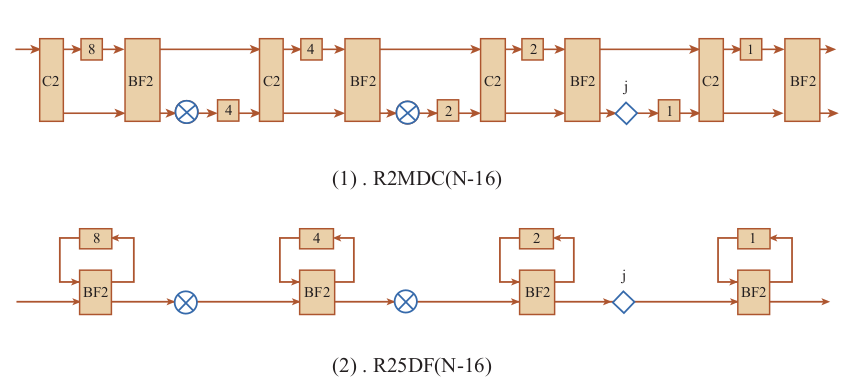
\includegraphics[width=0.5\linewidth]{Diagramas/types_FFT.png}
	\caption{Types of pipelined FFT archicectures for 16 points \cite{type_FFT_MIT}.}
	\label{fig:types_fft}
\end{figure*}



%%%%%%%%%
% Seccion
%%%%%%%%%
 
\section{Radix-$2^3$ FFT algorithm} \label{sec:equa}
The \textit{N}-point DFT of an input sequence $x[n]$ is defined as:

\begin{equation}
	X[k] = \sum_{n=0}^{N-1} x[n] \dot W_N^{nk}, \quad k=0,1,...,N-1
\end{equation}
where $W_N^{nk} = e^{-j\frac{2\pi}{N} nk}$. 

The FFT based on Cooley-Tukey algorithm is most commonly used to compute the DFT efficiently, this allows to reduce the number of operations from \textit{O($N^2$)} to \textit{O($Nlog_2N$)}. Direct computation of the DFT is basically inefficient, primarily because it does not exploit the symmetry and periodicity properties of the phase factor $W_N$, these two properties are:
\begin{align}
	&\text{Symmetry property: } W_N^{k+N/2} = -W_N^k	\\
	&\text{Periodicity property: } W_N^{k+N} = W_N^k
\end{align}

The development of computationally efficient algorithms for DFT is possible if a \textit{Divide and Conquer} approach is adopted. This approach is based on the decomposition of an \textit{N} point DFT into successively smaller DFTs, this means that the DFT is calculated as a series of $s=log_\rho N$ stages, where $\rho$ is the base of the \textit{radix}, e.g., in this work this factor is two, so the number of stages for 128 points is 7.

According to \cite{proakis_digital_nodate,oppenheim_tratamiento_2011}, There are two methods to design FFT algorithms: 
\paragraph{Decimation in time (DIT)}
In this method the \textit{N}-point data sequence $x[n]$ is split into two $N/2$-point data sequences, thus, is possible to obtain two different functions by decimating $x[n]$ by a factor of 2. The decimation of the data sequence can be repeated again, until the resulting sequences are reduced to one-point sequence. 
\paragraph{Decimation in frequency (DIF)}
This method is based on the divide-and-conquer technique, where the DFT formula is split into two summations, one of which involves the sum over the first $N/2$ data points and the second sum involves the last $N/2$ data points.


In each decomposition, the basic computing unit that processes the samples is called \textit{butterfly}. In general, each butterfly involves one complex multiplication and two complex additions. The main difference between DIT and DIF is the instant in which the multiplication by $W_N^\phi$ is computed, the input samples can be multiplied before or after the butterfly structure, as is depicted in Fig.\ref{fig:difdit}.




\begin{figure} [ht!]
	\centering
	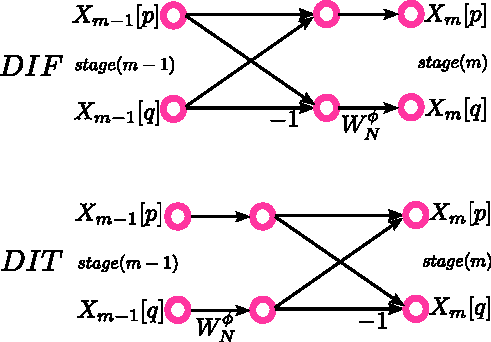
\includegraphics[width=0.65\linewidth]{Diagramas/miSeccionFiguras/DifDit.pdf}
	\caption{Basic butterflies computation in the decimation in time and frequency.}
	\label{fig:difdit}
\end{figure}

Another difference between the two methods is that the input samples in DIF algorithms are organized in natural order but the output are not in order, in which case a reordering circuit at the output is needed, in contrast with the DIT algorithms where the input sequence are not in order but the output is in natural order.

According to the methodology presented in \cite{proakis_digital_nodate}, it is possible to apply the mathematical expressions of \textit{radix-}$2^3$ DIF as is explain in \cite{jia_efficient_nodate}. These fundamental equations are describe in equation (\ref{eqn:radix}):

%%Ecuaciones RADIX
\begingroup
\allowdisplaybreaks
\begin{small}
\begin{align}\label{eqn:radix}
C_{8k+0} = \sum_{n=0}^{N/8-1} \bigg\{&[(x_n + x_{n+\frac{N}{2}}) + (x_{n+\frac{N}{4}} + x_{n+\frac{3N}{4}})] + 	   				    \\
&[(x_{n+\frac{N}{8}} + x_{n+\frac{5N}{8}}) + (x_{n+\frac{3N}{8}} + x_{n+\frac{7N}{8}})] \bigg\} W_N^{0n} W_{N/8}^ {nk}     \nonumber\\
%	
C_{8k+4} = \sum_{n=0}^{N/8-1} \bigg\{&[(x_n + x_{n+\frac{N}{2}}) + (x_{n+\frac{N}{4}} + x_{n+\frac{3N}{4}})] - 			   \nonumber\\
&[(x_{n+\frac{N}{8}} + x_{n+\frac{5N}{8}}) + (x_{n+\frac{3N}{8}} + x_{n+\frac{7N}{8}})] \bigg\} W_N^{4n} W_{N/8}^ {nk}     \nonumber\\
%
C_{8k+2} = \sum_{n=0}^{N/8-1} \bigg\{&[(x_n + x_{n+\frac{N}{2}}) - (x_{n+\frac{N}{4}} + x_{n+\frac{3N}{4}})] -j 		   \nonumber\\
&[(x_{n+\frac{N}{8}} + x_{n+\frac{5N}{8}}) - (x_{n+\frac{3N}{8}} + x_{n+\frac{7N}{8}})] \bigg\} W_N^{2n} W_{N/8}^ {nk}     \nonumber\\
%
C_{8k+6} = \sum_{n=0}^{N/8-1} \bigg\{&[(x_n + x_{n+\frac{N}{2}}) - (x_{n+\frac{N}{4}} + x_{n+\frac{3N}{4}})] +j			   \nonumber\\
&[(x_{n+\frac{N}{8}} + x_{n+\frac{5N}{8}}) - (x_{n+\frac{3N}{8}} + x_{n+\frac{7N}{8}})] \bigg\} W_N^{6n} W_{N/8}^ {nk}     \nonumber\\
%
C_{8k+1} = \sum_{n=0}^{N/8-1} \bigg\{&[(x_n - x_{n+\frac{N}{2}}) -j (x_{n+\frac{N}{4}} - x_{n+\frac{3N}{4}})] + W_N^{N/8}  \nonumber\\
&[(x_{n+\frac{N}{8}} - x_{n+\frac{5N}{8}}) -j (x_{n+\frac{3N}{8}} - x_{n+\frac{7N}{8}})] \bigg\} W_N^{n} W_{N/8}^ {nk}     \nonumber\\
%
C_{8k+5} = \sum_{n=0}^{N/8-1} \bigg\{&[(x_n - x_{n+\frac{N}{2}}) -j (x_{n+\frac{N}{4}} - x_{n+\frac{3N}{4}})] - W_N^{N/8}  \nonumber\\
&[(x_{n+\frac{N}{8}} - x_{n+\frac{5N}{8}}) -j (x_{n+\frac{3N}{8}} - x_{n+\frac{7N}{8}})] \bigg\} W_N^{5n} W_{N/8}^ {nk}    \nonumber\\
%
C_{8k+3} = \sum_{n=0}^{N/8-1} \bigg\{&[(x_n - x_{n+\frac{N}{2}}) +j (x_{n+\frac{N}{4}} - x_{n+\frac{3N}{4}})] + W_N^{3N/8} \nonumber\\
&[(x_{n+\frac{N}{8}} - x_{n+\frac{5N}{8}}) +j (x_{n+\frac{3N}{8}} - x_{n+\frac{7N}{8}})] \bigg\} W_N^{3n} W_{N/8}^ {nk}    \nonumber\\
%
C_{8k+7} = \sum_{n=0}^{N/8-1} \bigg\{&[(x_n - x_{n+\frac{N}{2}}) +j (x_{n+\frac{N}{4}} + x_{n+\frac{3N}{4}})] - W_N^{3N/8} \nonumber\\
&[(x_{n+\frac{N}{8}} - x_{n+\frac{5N}{8}}) +j (x_{n+\frac{3N}{8}} - x_{n+\frac{7N}{8}})] \bigg\} W_N^{7n} W_{N/8}^ {nk}    \nonumber	
\end{align}
\end{small}
\endgroup


Fig. \ref{fig:8ponits_df} and Fig. \ref{fig:8ponits_dfg} show the equivalent diagram of interconnections and data flows from the equations presented in (\ref{eqn:radix}).

%The use of higher value radices lead to different amount of rotators. If we compare the quantity of rotators of an architecture \textit{radix-}$2$ FFT with an architecture \textit{radix-}$2^k$ FFT, this last has less number of phase factors.

\begin{figure}[ht] 
	\centering
	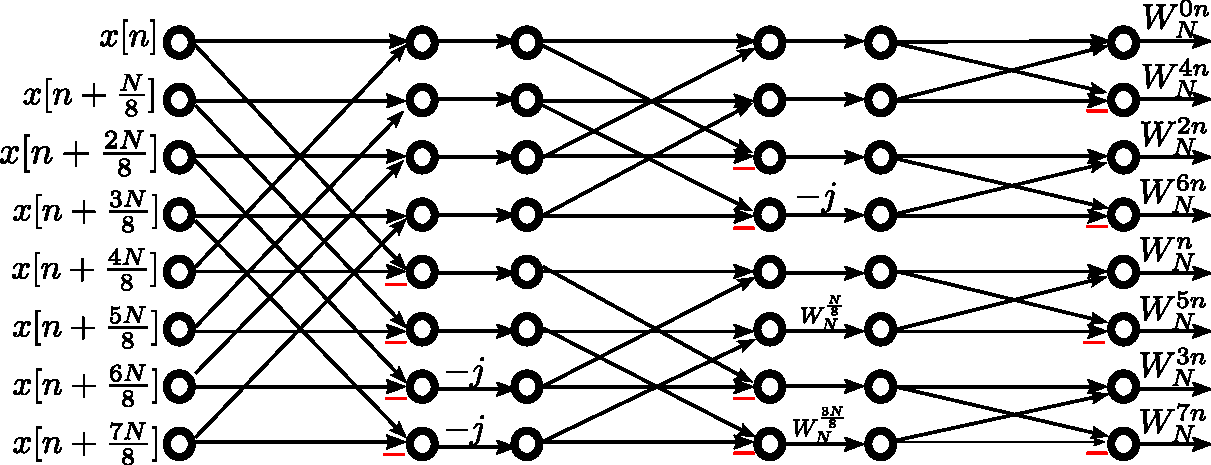
\includegraphics[width=\linewidth]{Diagramas/miSeccionFiguras/8PuntosRadix8Conexion.pdf}
	\caption{Structure of interconnection for \textit{radix-}$2^3$ DIF DFT.}
	\label{fig:8ponits_df}
\end{figure}

\begin{figure} [ht]
	\centering
	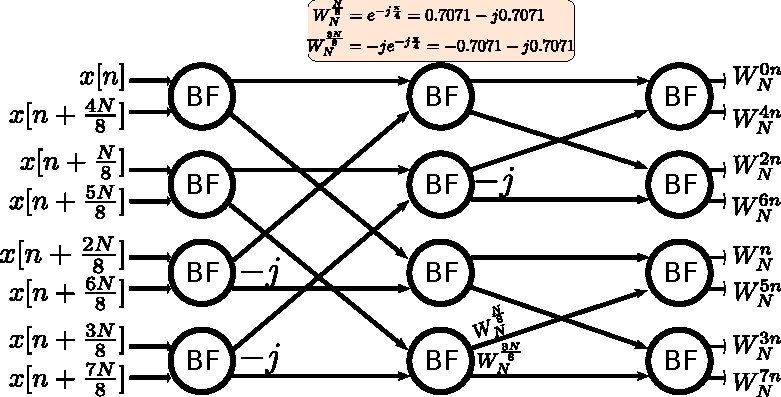
\includegraphics[width=\linewidth]{Diagramas/miSeccionFiguras/8PuntosRadix8Burbujas.pdf}
	\caption{Data flow graph (DFG) based in equations (\ref{eqn:radix}).}
	\label{fig:8ponits_dfg}
\end{figure}

\subsection{16 points DFT}
The next step is to find the suitable rotator factors for the 16 point DFT, the equations in (\ref{eqn:radix}) are essential for this design and they were evaluated to get $C_{8k+i} = \sum_{n=0}^{16/8-1} \{ \cdot \}, $ for $k=0,1$. The structure for the 16 point DFT is described in Fig. \ref{fig:16points_df} and Fig. \ref{fig:16points_dfg}. 

\begin{figure} [ht]
	\centering
	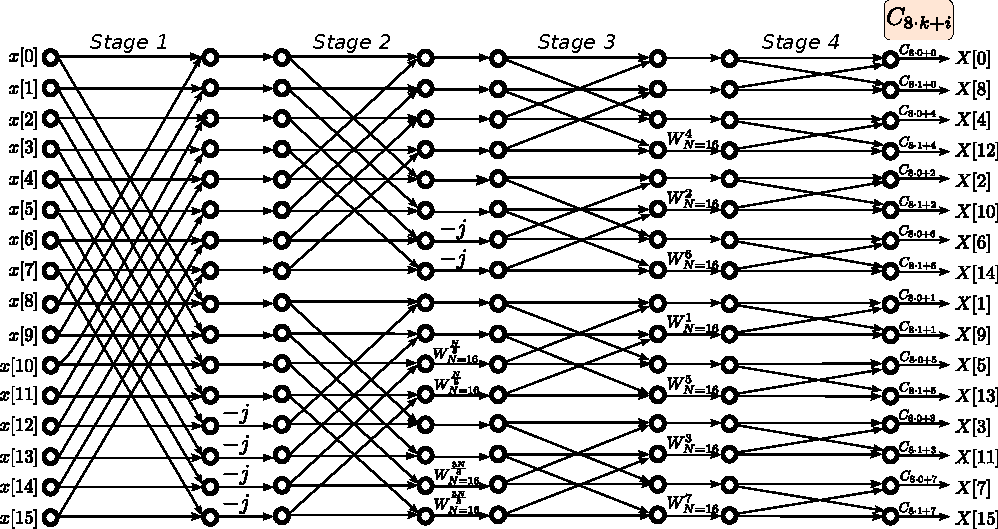
\includegraphics[width=\linewidth]{Diagramas/miSeccionFiguras/16PuntosRadix8Conexion.pdf}
	\caption{Flow graph of a \textit{radix-}$2^3$ 16-point DIF DFT}
	\label{fig:16points_df}
\end{figure}

\begin{figure} [ht]
	\centering
	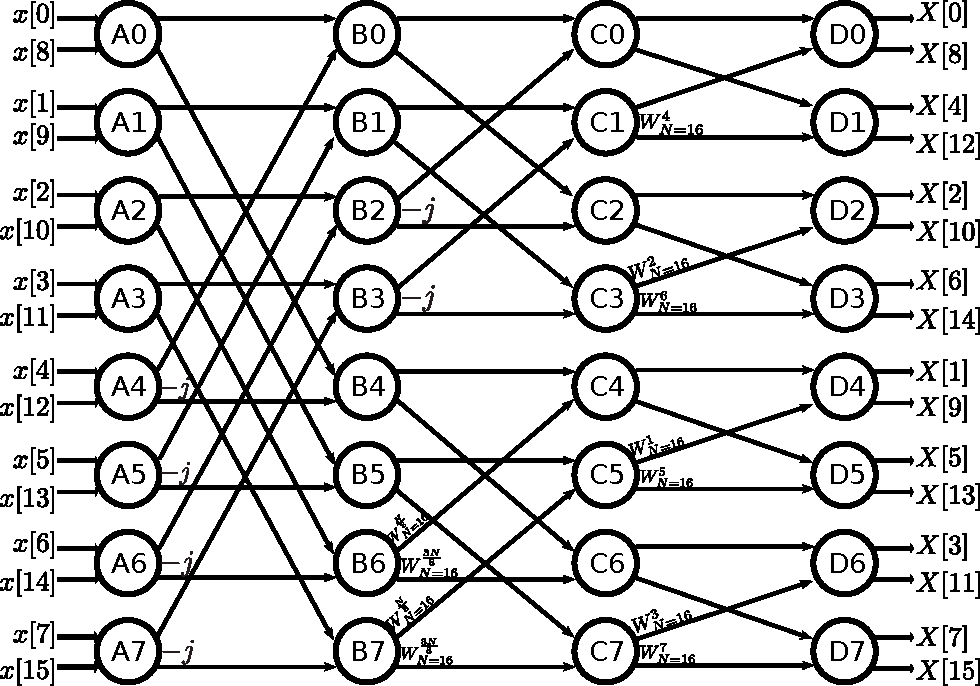
\includegraphics[width=\linewidth]{Diagramas/miSeccionFiguras/16PuntosRadix8Burbujas.pdf}
	\caption{Data flow graph (DFG) for a \textit{radix-}$2^3$ 16-point DIF DFT}
	\label{fig:16points_dfg}
\end{figure}

\subsection{128 points DFT}
With these first approaches is possible the application of the divide and conquer strategy by decomposing the 128-point DFT and calculating each coefficient $C_{8k+i} = \sum_{n=0}^{128/8-1} \{ \cdot \}, $ for $k=0,1,...,(128/8)-1$, this way a  chain sequence of butterflies is obtained together with its corresponding rotation factor and the correct index of the samples in which they must be added or multiplied. Using this technique is possible to do a subdivision of butterflies stages, as is shown in Fig. \ref{fig:128_block_descomp}, the decomposition of the 128 point DFT involve three stages of butterflies, to finally arrive to a set of eight 16 point DFTs. Finally, Fig. \ref{fig:128ponits_conn} shows the complete architecture for the  \textit{radix-}$2^3$ 128-point DIF DFT with a total of seven stages where each stage is contains 64 butterflies of radix-2 base.

\begin{figure} [ht]
	\centering
	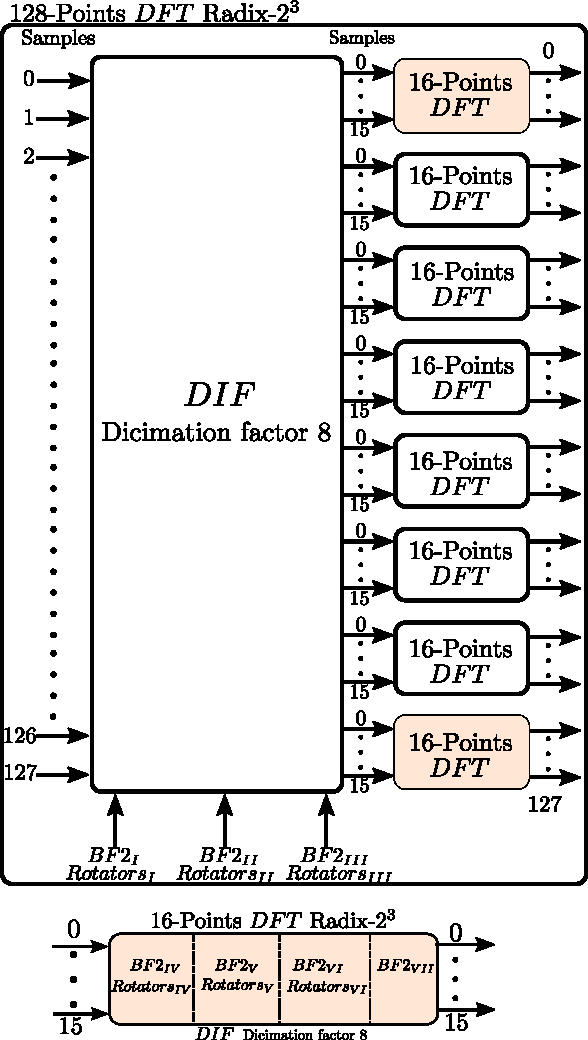
\includegraphics[width=\linewidth]{Diagramas/miSeccionFiguras/BloquesDft.pdf}
	\caption{Decomposing a \textit{radix-}$2^3$ 128-point DFT.}
	\label{fig:128_block_descomp}
\end{figure}



%
%With the DFT's previous decomposition is possible to get whole the coefficients $C_{8k+i}$ that represent the samples in frequency $X[k]$ obtained from a combination of the different instances of $x[n]$. This method take us to apply step by step the equation (\ref{eqn:radix}) to our design and finally arrive to the definitive architecture, the Fig. \ref{fig:128ponits_conn} shows us a \textit{radix-}$2^3$ 128-point DIF DFT with a total of seven stages where each stage is building with 64 butterflies of radix-2 base.

\begin{figure} 
	\centering
	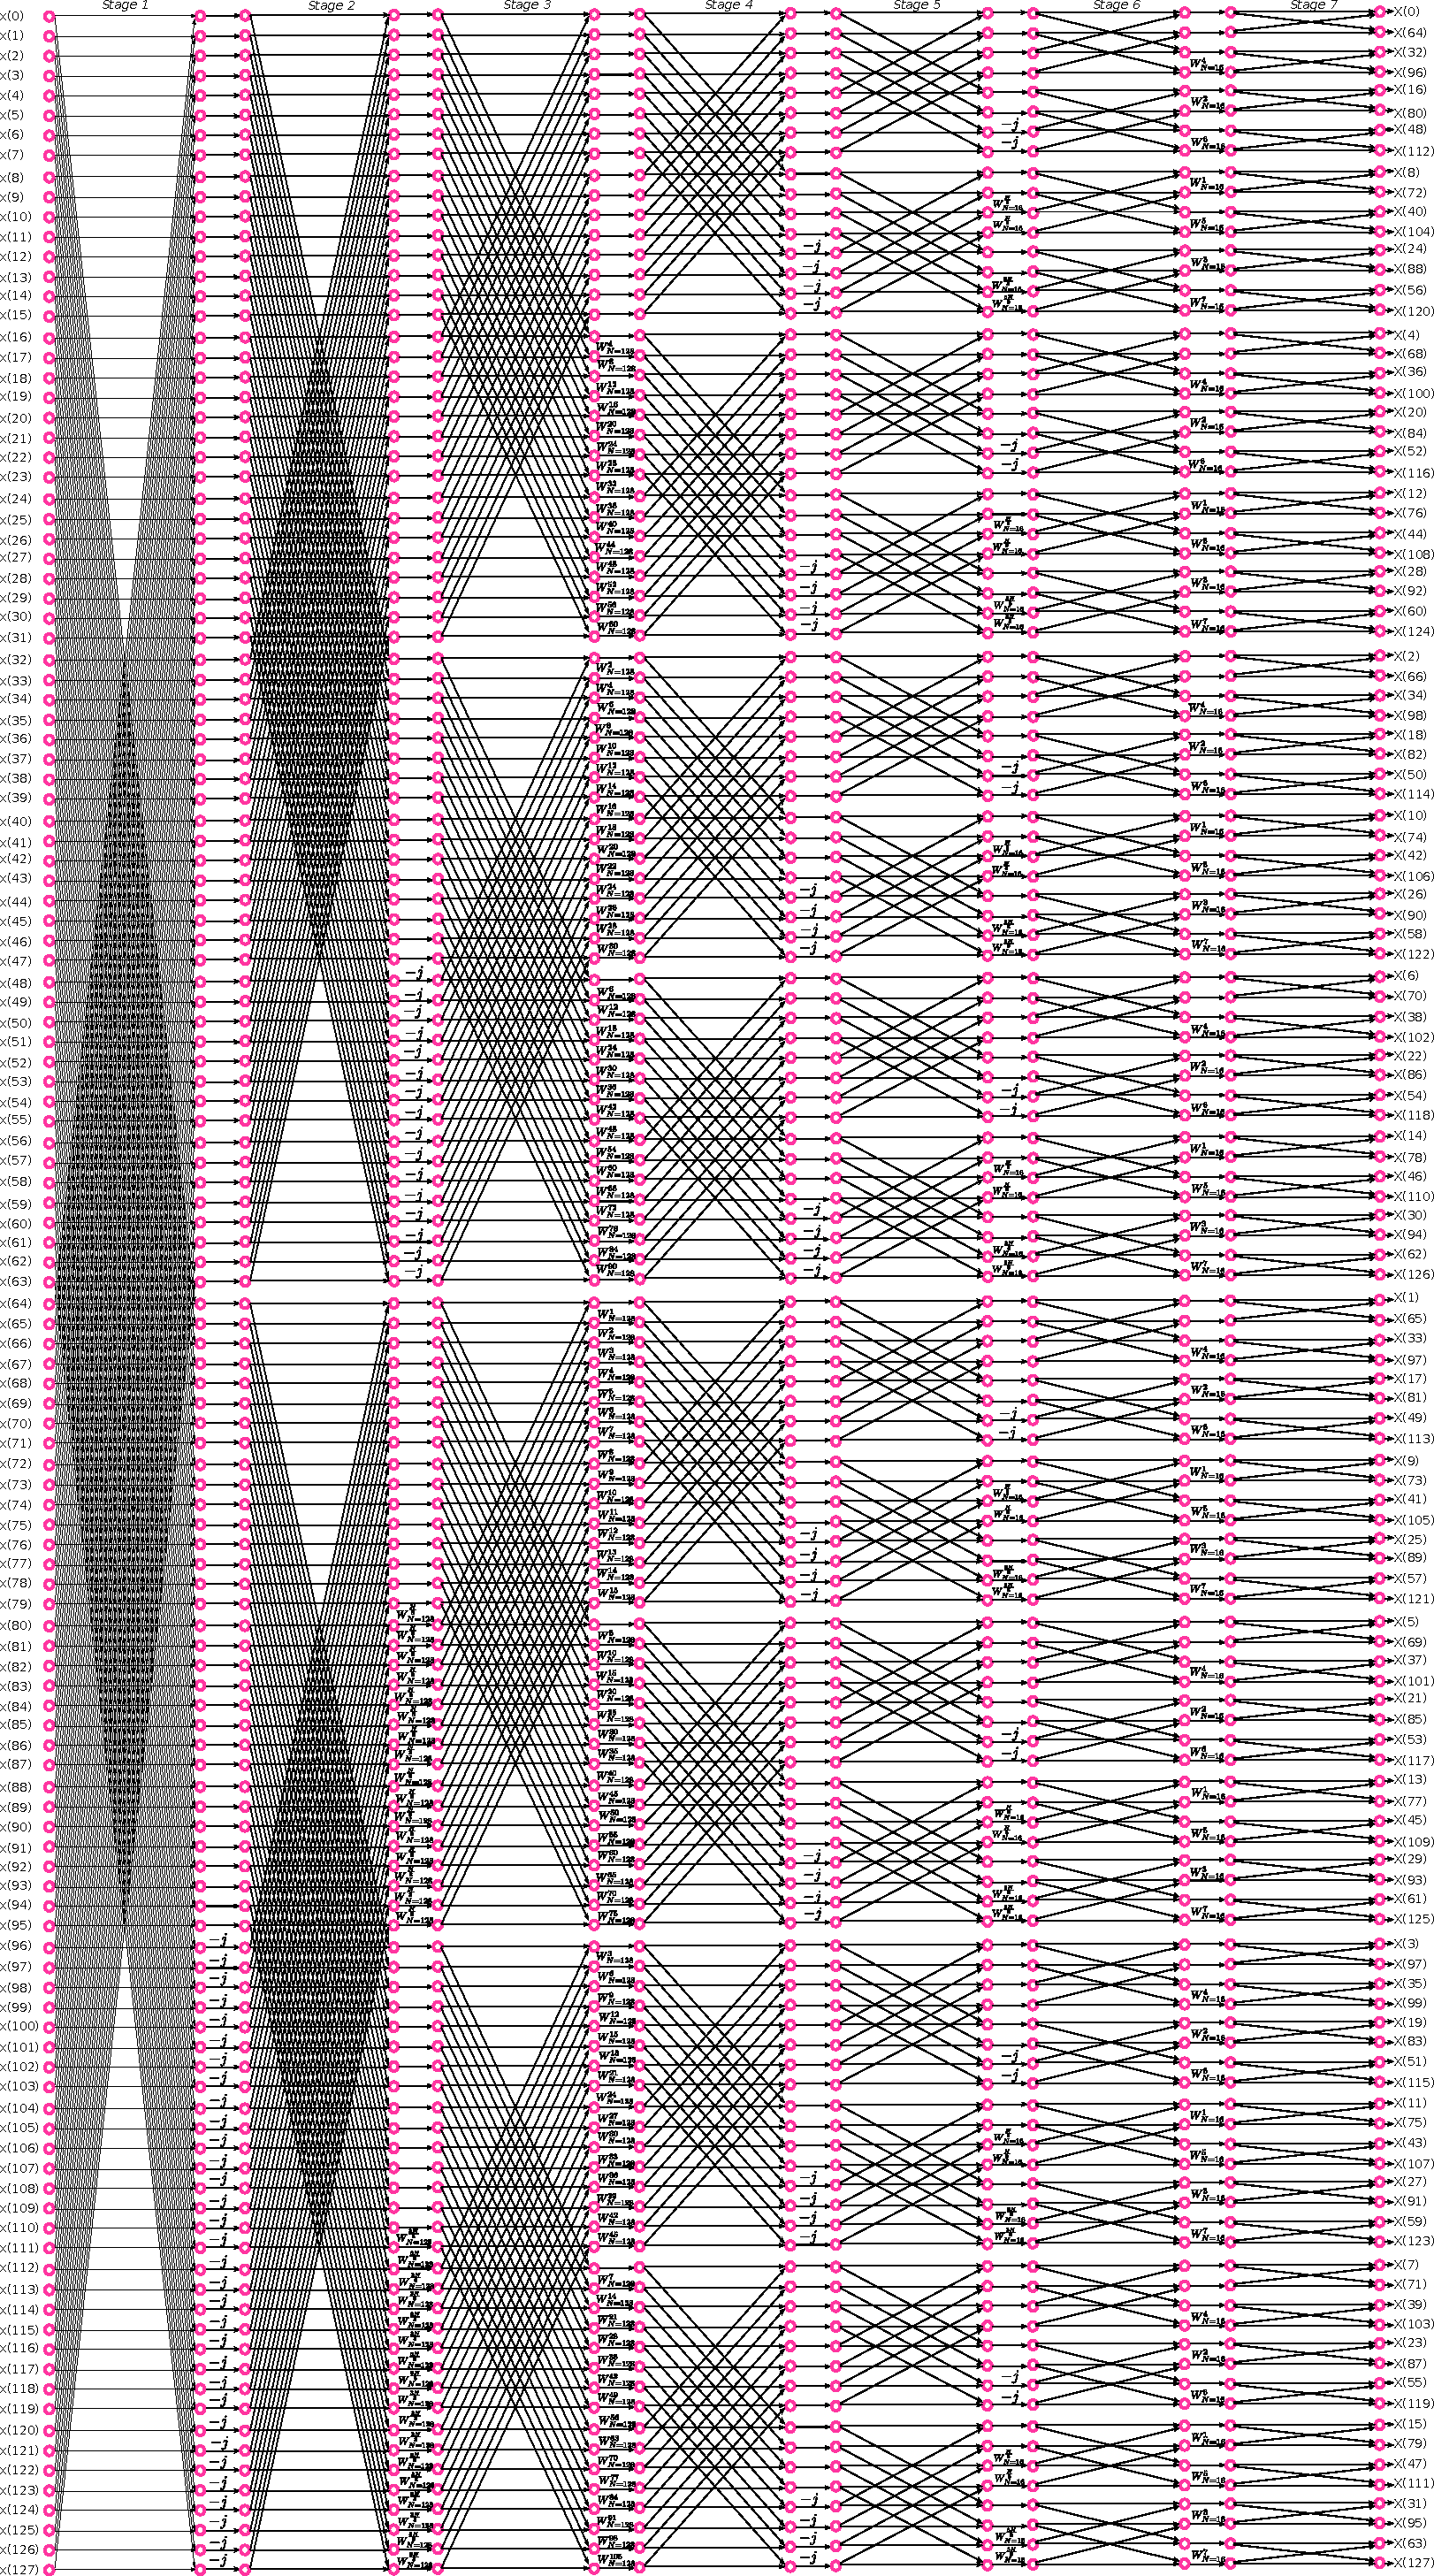
\includegraphics[width=\linewidth]{Diagramas/miSeccionFiguras/128PuntosRadix8Conexion.pdf}
	\caption{Flow graph of a \textit{radix-}$2^3$ 128-point DIF DFT}
	\label{fig:128ponits_conn}
\end{figure}



%%%%%%%%%%
%% Seccion
%%%%%%%%%%
 


\section{Design of a FFT architecture via folding transformation} \label{sec:16points}
In this section, the architecture proposed in \cite{ayinala_pipelined_2012} together with the folding transformation and register minimization techique described in \cite{folding_parhi_book} is used to obtain a 16-point DIF FFT 4-parallel architecture, then, the same method is extended  to achieve a 128-point DIF FFT 4-parallel architecture.




%%%%%%%%%%%%%
%% Subseccion
%%%%%%%%%%%%%
\subsection{4-Parallel radix-$2^3$ 16-Points}
The flow graph of a 16-point DIF FFT radix-$2^3$ with main base radix-2 is shown in Fig. \ref{fig:16points_df}. The graph is divided into four stages, each of them consist of a set of butterflies and multipliers. The twiddle factor between the stages indicates a multiplication by $W^k_N$, where $W_N$ denotes the \textit{N}th root of unity, with its exponent evaluated modulo N. This can be represented as a DFG as shown in Fig. \ref{fig:16points_dfg}, where the nodes represents the butterfly computations of the radix-2 FFT algorithm. 

The folding transformation is used on the DFG to derive a pipelined architecture, to do this a folding set is needed. A folding set is an ordered set of operations executed by the same functional unit, each folding set contains K entries, where K is called the folding factor. The operation in the \textit{j}th position within the folding set (where goes from $0$ to $K-1$) is executed by the functional unit during the time partition, this term is called the folding order.

In order to derive the folding equations a node graph is needed, where an edge $e$ is consider to connect the nodes \textit{U} and \textit{V} with $w(e)$ delays. Let the executions of the \textit{l}th iteration of the nodes \textit{U} and \textit{V} be scheduled at the time units $Kl+u$ and $Kl+v$ respectively, where $u$ and $v$ are the folding orders of the nodes \textit{U} and \textit{V}, respectively. The folding equation for the edge $e$ is:
\begin{equation}\label{eqn:fold_equation}
D_F(U \to V) = Kw(e)-P_U+v-u
\end{equation}

where $P_U$ is the number of pipeline stages in the hardware unit which executes the node U.

Consider folding of the the DFG in Fig. \ref{fig:16points_dfg} with the folding sets:
\begin{align*}%\label{eq:foldingset_16}
A&= \{ A0,A2,A4,A6 \}  & A'&= \{ A1,A3,A5,A7 \} \\
B&=\{ B1,B3,B0,B2 \}   &B'&=\{ B5,B7,B4,B6 \} 	\\
C&=\{ C2,C1,C3,C0 \}   &C'&=\{ C6,C5,C7,C4 \} 	\\ 
D&=\{ D3,D0,D2,D1 \}   &D'&=\{ D7,D4,D6,D5 \}  
\end{align*}

Assuming that the butterfly operations do not have any pipeline stages ($P_A=P_B=P_C=P_D=0$), the folding equations can be derived for all edges,
thus, the expression \textit{without retiming} can be obtained from (\ref{eqn:fold_equation}) 

%%% Ecuaciones de folding sin pipe
\begin{small}
\begin{align*}%%\label{eqn:fold_equation} 
D_F(A0\to B0)&=2 &  D_F(A0\to B4)&=2\\
D_F(A1\to B1)&=0 &  D_F(A1\to B5)&=0\\
D_F(A2\to B2)&=2 &  D_F(A2\to B6)&=2\\
D_F(A3\to B3)&=-1& D_F(A3\to B7)&=-1\\
D_F(A4\to B0)&=0 &  D_F(A4\to B4)&=0\\
D_F(A5\to B1)&=-1& D_F(A5\to B5)&=-1\\
D_F(A6\to B2)&=0 &  D_F(A6\to B6)&=0\\
D_F(A7\to B3)&=-2& D_F(A7\to B7)&=-2\\
D_F(B0\to C0)&=1 &  D_F(B0\to C2)&=-2\\
D_F(B1\to C1)&=1 &  D_F(B1\to C3)&=2\\
D_F(B2\to C0)&=0 &  D_F(B2\to C2)&=-3\\
D_F(B3\to C1)&=0 &  D_F(B3\to C3)&=1\\
D_F(B4\to C4)&=1 &  D_F(B4\to C6)&=-2\\
D_F(B5\to C5)&=1 &  D_F(B5\to C7)&=2\\
D_F(B6\to C4)&=0 &  D_F(B6\to C6)&=-3\\
D_F(B7\to C5)&=0 &  D_F(B7\to C7)&=1\\
D_F(C0\to D0)&=-2& D_F(C0\to D1)&=0\\
D_F(C1\to D0)&=0 &  D_F(C1\to D1)&=2\\
D_F(C2\to D2)&=2 &  D_F(C2\to D3)&=0\\
D_F(C3\to D2)&=0 &  D_F(C3\to D3)&=-2\\
D_F(C4\to D4)&=-2&  D_F(C4\to D5)&=0\\
D_F(C5\to D4)&=0 &  D_F(C5\to D5)&=2\\
D_F(C6\to D6)&=2 &  D_F(C6\to D7)&=0\\
D_F(C7\to D6)&=0 &  D_F(C7\to D7)&=-2
\end{align*}
\end{small}
For the folded system to be realizable, $D_F(U\to V)\geq0$ must hold for all the edges in the DFG. Retimming and/or pipeline can be applied to satisfy this property, if the DFG in Fig. \ref{fig:16points_dfg} is pipelined/retimmed as shown in Fig. \ref{fig:dfg_16_ret} the system is realizable and the folded delays for the edges are given by the equations that represent a folding set \textit{with retiming}.

\begin{figure} 
\centering
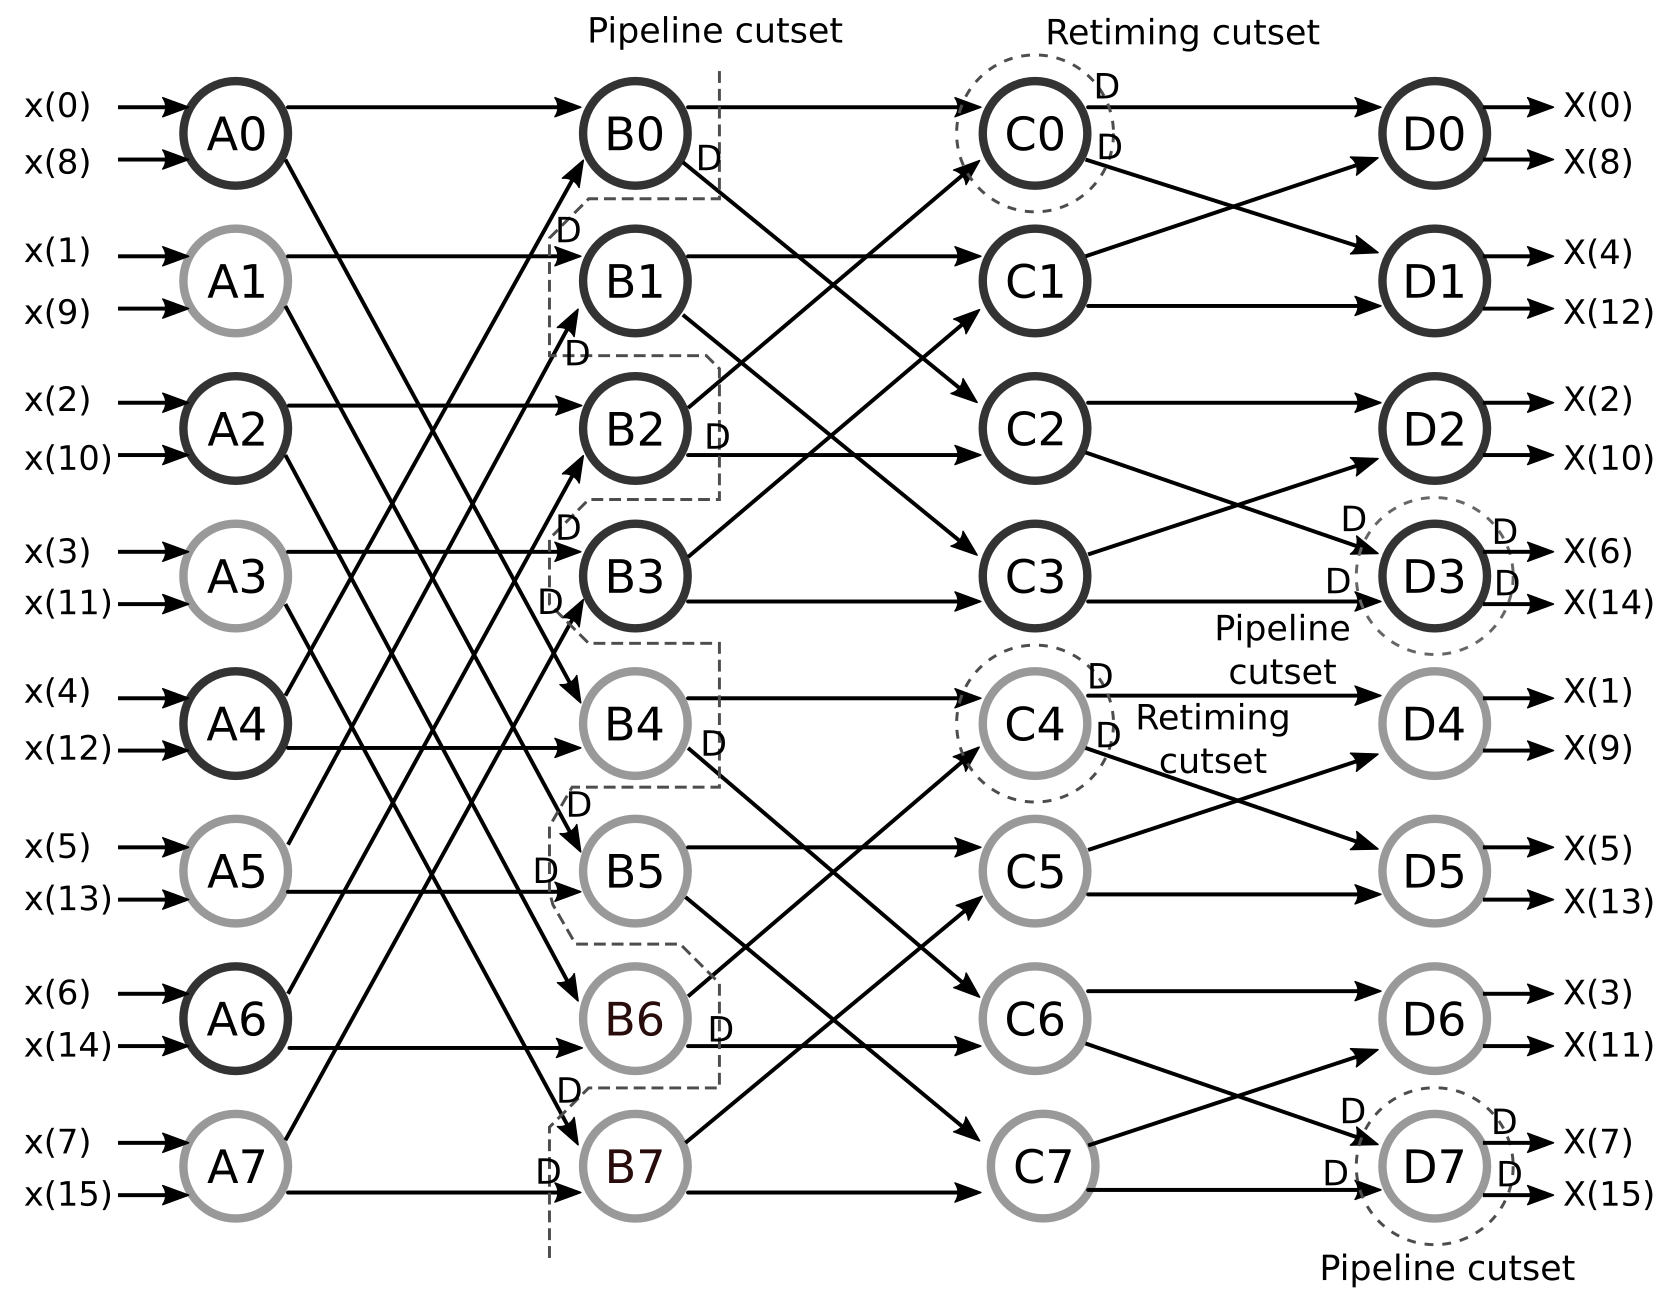
\includegraphics[width=\linewidth]{Diagramas/16points_dfg_ret.png}
\caption{Data Flow graph (DFG) of a radix-2 16-point DIF FFT with retiming and pipeline.}
\label{fig:dfg_16_ret}
\end{figure}
%%%ecuaciones de folding con pipe
\begin{small}
\begin{align}\label{eqn:ConRetiming} 
D_F(A0\to B0)&=2 &  D_F(A0\to B4)&=2 		 \\
D_F(A1\to B1)&=4 &  D_F(A1\to B5)&=4\nonumber\\
D_F(A2\to B2)&=2 &  D_F(A2\to B6)&=2\nonumber\\
D_F(A3\to B3)&=3 &  D_F(A3\to B7)&=3\nonumber\\
D_F(A4\to B0)&=0 &  D_F(A4\to B4)&=0\nonumber\\
D_F(A5\to B1)&=3 &  D_F(A5\to B5)&=3\nonumber\\
D_F(A6\to B2)&=0 &  D_F(A6\to B6)&=0\nonumber\\
D_F(A7\to B3)&=2 &  D_F(A7\to B7)&=2\nonumber\\
D_F(B0\to C0)&=1 &  D_F(B0\to C2)&=2\nonumber\\
D_F(B1\to C1)&=1 &  D_F(B1\to C3)&=2\nonumber\\
D_F(B2\to C0)&=0 &  D_F(B2\to C2)&=1\nonumber\\
D_F(B3\to C1)&=0 &  D_F(B3\to C3)&=1\nonumber\\
D_F(B4\to C4)&=1 &  D_F(B4\to C6)&=2\nonumber\\
D_F(B5\to C5)&=1 &  D_F(B5\to C7)&=2\nonumber\\
D_F(B6\to C4)&=0 &  D_F(B6\to C6)&=1\nonumber\\
D_F(B7\to C5)&=0 &  D_F(B7\to C7)&=1\nonumber\\
D_F(C0\to D0)&=2 &  D_F(C0\to D1)&=4\nonumber\\
D_F(C1\to D0)&=0 &  D_F(C1\to D1)&=2\nonumber\\
D_F(C2\to D2)&=2 &  D_F(C2\to D3)&=4\nonumber\\
D_F(C3\to D2)&=0 &  D_F(C3\to D3)&=2\nonumber\\
D_F(C4\to D4)&=2 &  D_F(C4\to D5)&=4\nonumber\\
D_F(C5\to D4)&=0 &  D_F(C5\to D5)&=2\nonumber\\
D_F(C6\to D6)&=2 &  D_F(C6\to D7)&=4\nonumber\\
D_F(C7\to D6)&=0 &  D_F(C7\to D7)&=2\nonumber
\end{align}
\end{small}

The number of registers required to implement the folding equations in (\ref{eqn:ConRetiming}) is 80, in order to minimize the number of registers  the register minimization technique is needed. 
If we let the output of node $A0$ be $y_{(0)}$ and $y_{(8)}$ and the output of the node A1 be $y_{(1)}$ and $y_{(9)}$, applying this successively with the rest of the nodes A we can obtain the linear life time chart for this stage in Fig. \ref{fig:tab-life-a}. Applying this criteria to the rest of the stages we can obtain the life time chart \ref{fig:tab-life-b} and \ref{fig:tab-life-c} for the outputs of the nodes B and C respectively, we can see that the numbers of maximum registers in each stage are 8, 4 and 8 respectively, therefore the number of registers is reduced from 80 to 20. More information about this method can be found on \cite{folding_parhi_book}.
\begin{figure}[t!]
\centering
 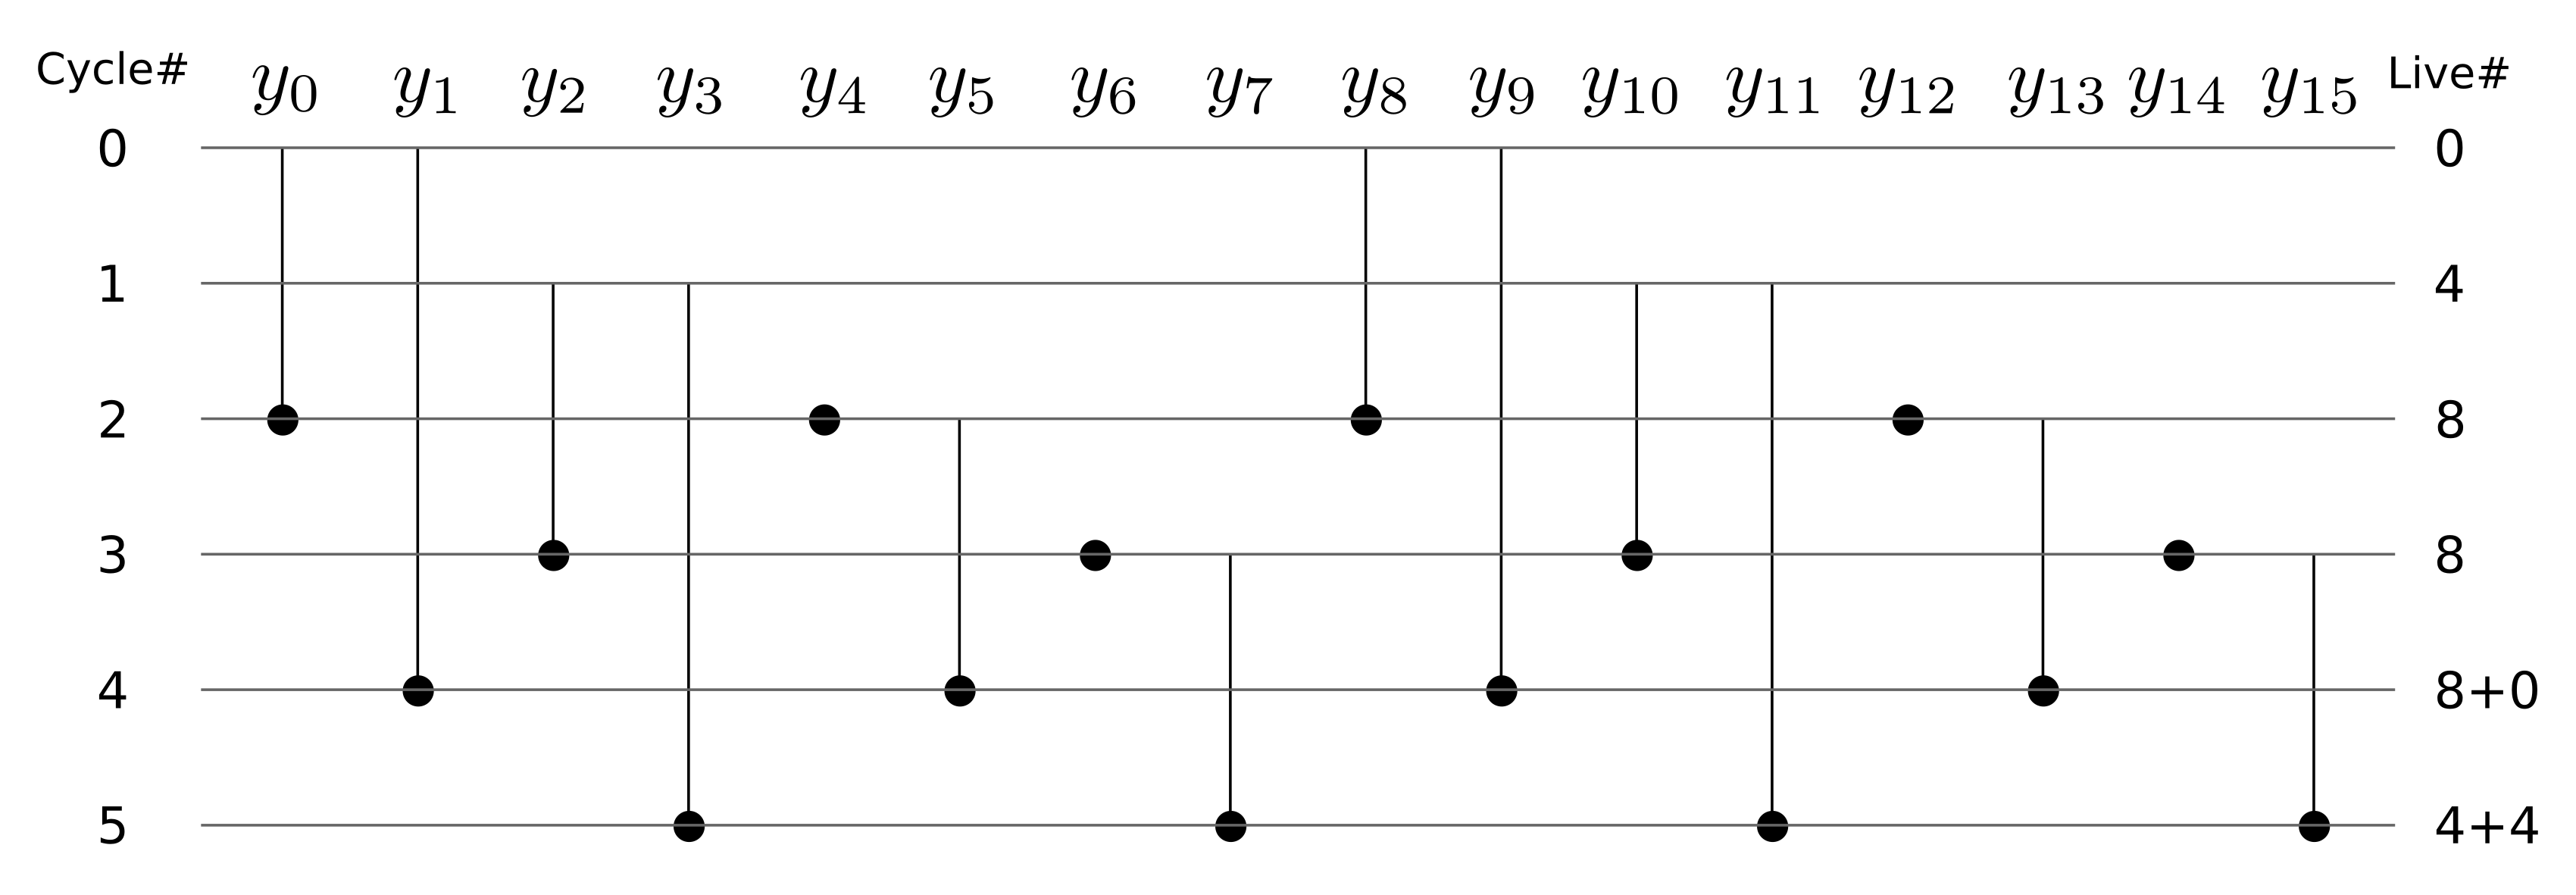
\includegraphics[width=\linewidth]{Diagramas/life_chart_a.png}
\caption{Linear lifetime chart for the variables $y_{(0)}, y_{(1)},...,y_{(15)}$ for a 16-point FFT architecture.}
\label{fig:tab-life-a}
\end{figure}
\begin{figure}[t!]
\centering
 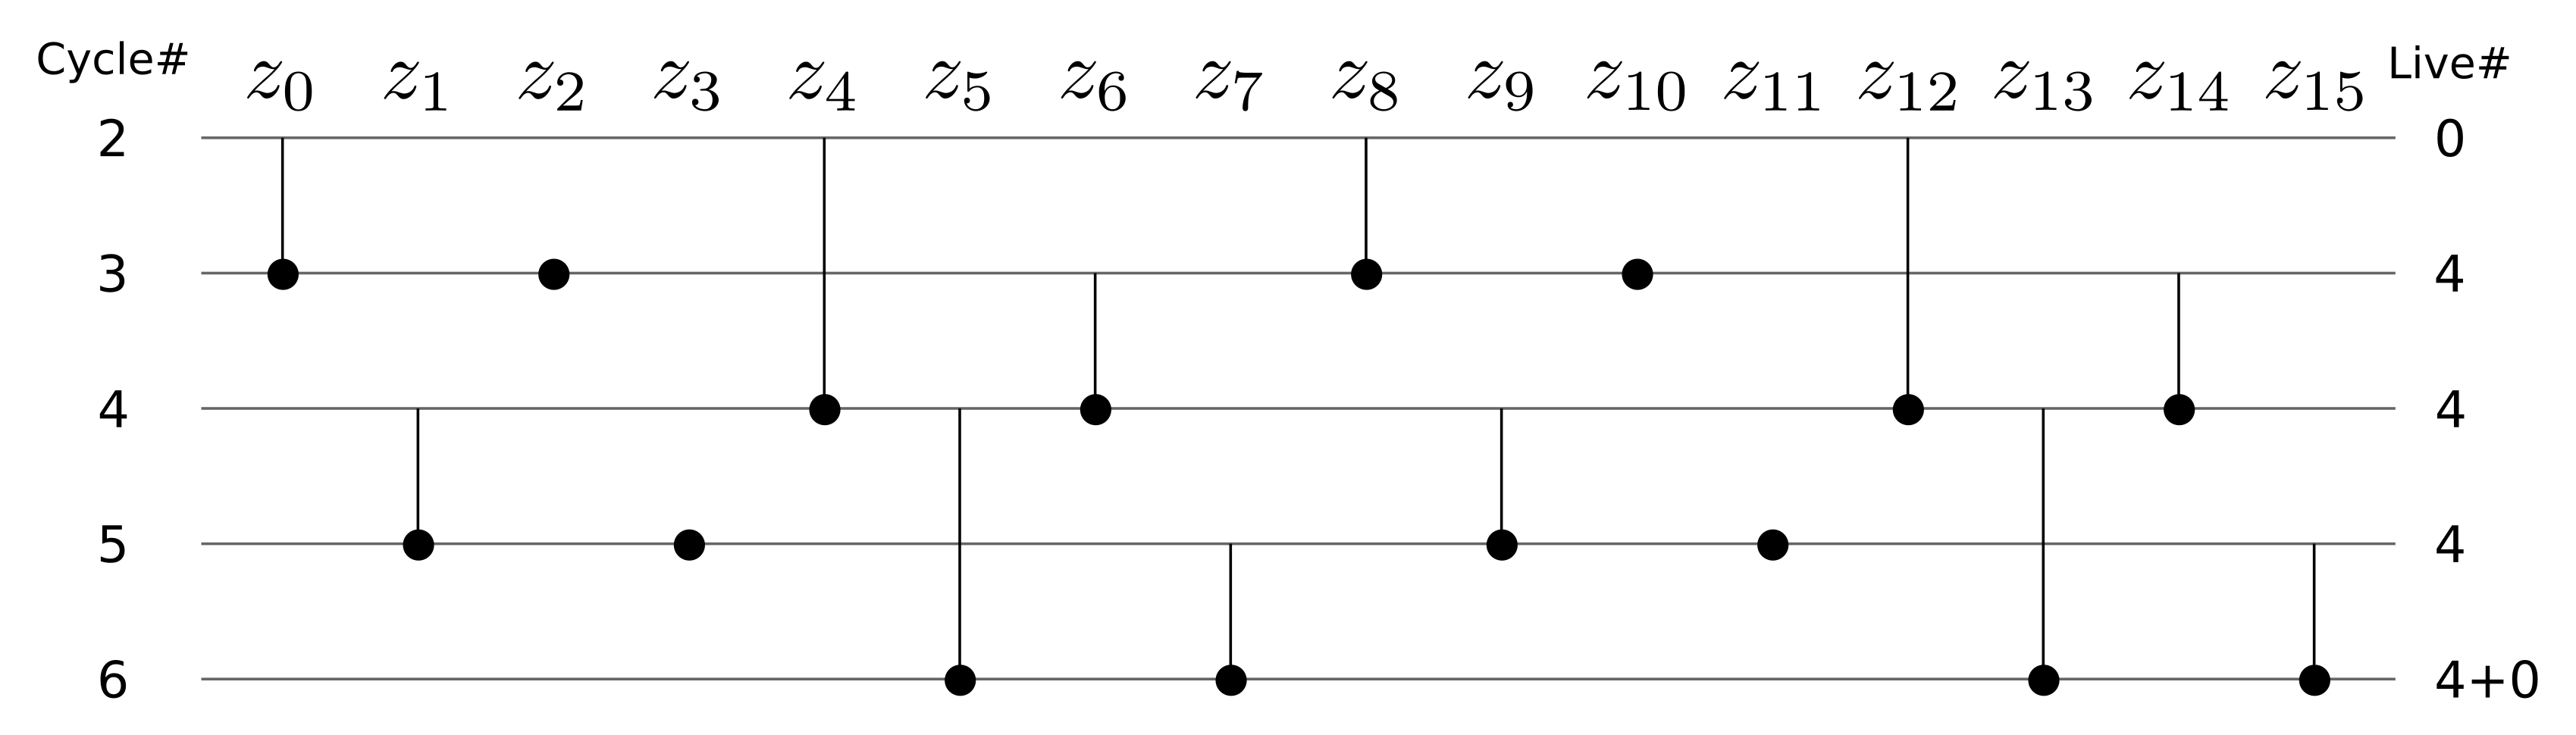
\includegraphics[width=\linewidth]{Diagramas/life_chart_b.png}
\caption{Linear lifetime chart for the variables $z_{(0)}, z_{(1)},...,z_{(15)}$ for a 16-point FFT architecture.}
\label{fig:tab-life-b}
\end{figure}
\begin{figure}[t!]
\centering
 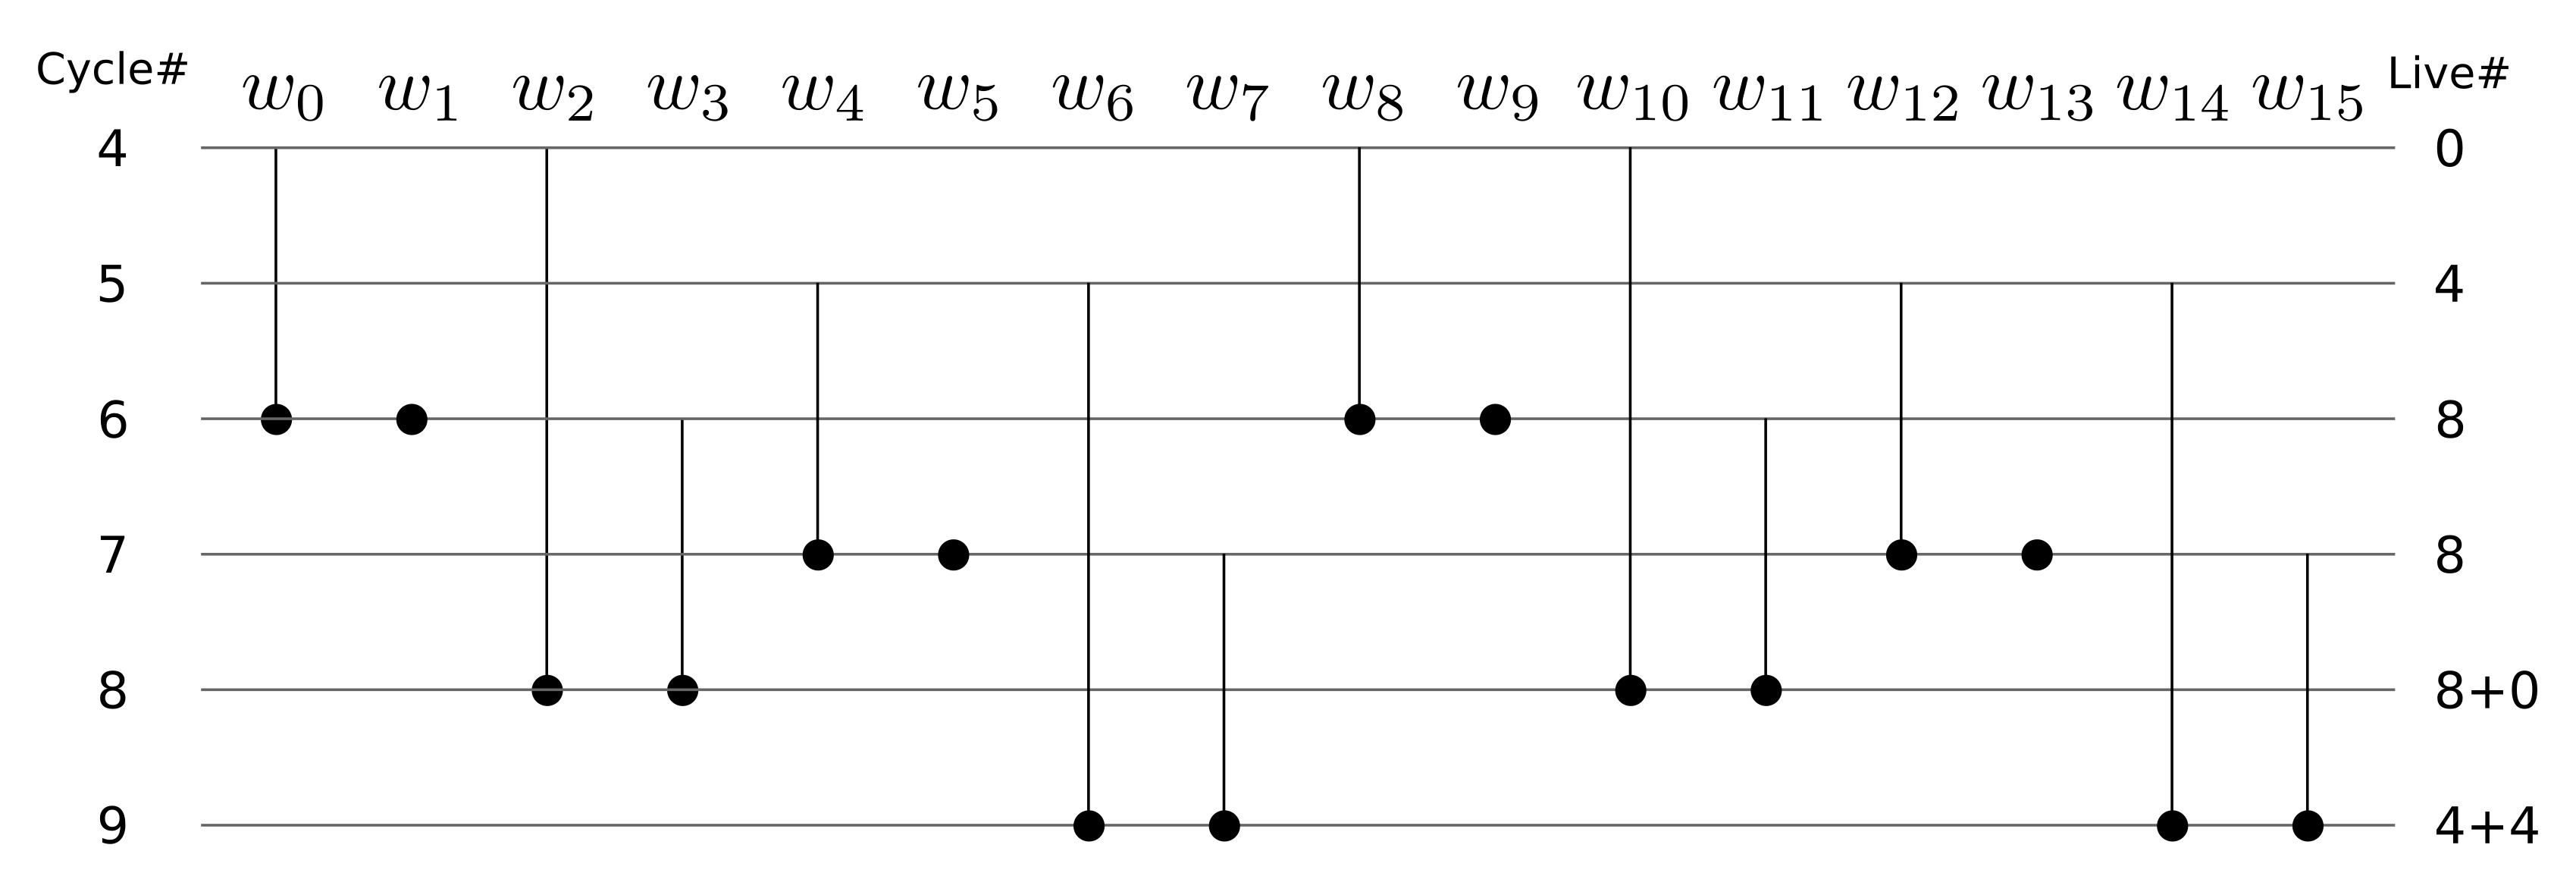
\includegraphics[width=\linewidth]{Diagramas/life_chart_c.png}
\caption{Linear lifetime chart for the variables $w_{(0)}, w_{(1)},...,w_{(15)}$ for a 16-point FFT architecture.}
\label{fig:tab-life-c}
\end{figure}

The register allocation tables for the lifetime charts are shown in Fig. \ref{fig:tab-aloc-a}, \ref{fig:tab-aloc-b} and \ref{fig:tab-aloc-c} for stage 1, 2 and 3 respectively. In the Fig. \ref{fig:folding16_stage1} and \ref{fig:folding16_stage2} is shown the designations of registers for the stage 1 and 2 respectively used in the allocation tables, the designation for stage 3 are similar for stage 1. The folded architecture in Fig. \ref{ fig:folding_16_arch} is synthesized using the folding equations and the register allocation tables. The dataflow for each stage can be see in Tab. \ref{tab:folding16_mux}, the control signal for stage 1 and 2 can be implemented by dividing the clock signal to 4 and 2 respectively, for stage 3 the control signal is the same that the stage 1.

The inputs of each folding node are represented with a matrix where the values in the same column are data that flow in parallel and values in the same row flow through the same path in consecutive clock cycles. The first two rows represents the inputs of the superior BF and the others two represents the input of the inferior BF. 
The same criteria is used for represent the constants of rotators, where each number $k$ of the matrix represent a multiplication by $W^k_N$.

\begin{figure} 
\centering
 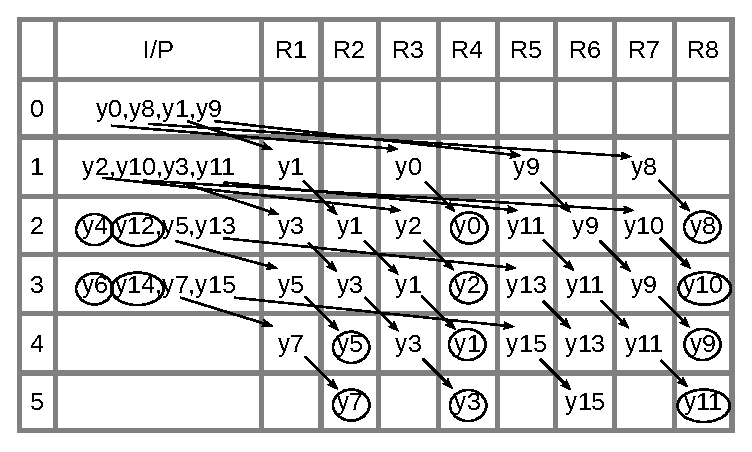
\includegraphics[width=0.9\linewidth]{Diagramas/tab_life_a.eps}
\caption{Register allocation table for the data represented in \ref{fig:tab-life-a}}
\label{fig:tab-aloc-a}
\end{figure}
\begin{figure} 
\centering
 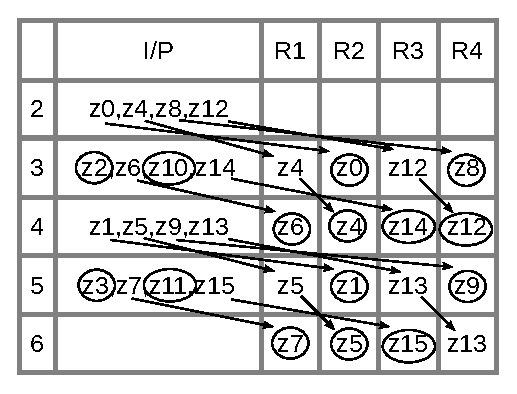
\includegraphics[width=0.63\linewidth]{Diagramas/tab_life_b.eps}
\caption{Register allocation table for the data represented in \ref{fig:tab-life-b}}
\label{fig:tab-aloc-b}
\end{figure}
\begin{figure} 
\centering
 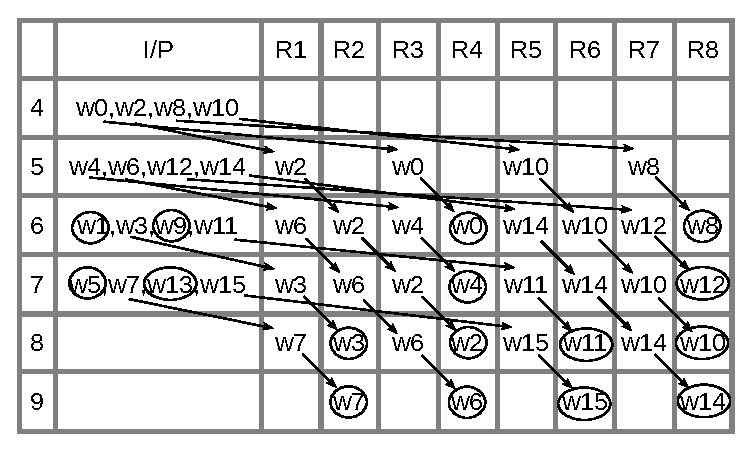
\includegraphics[width=0.95\linewidth]{Diagramas/tab_life_c.eps}
\caption{Register allocation table for the data represented in \ref{fig:tab-life-c}}
\label{fig:tab-aloc-c}
\end{figure}


\begin{table*}  
    \centering
    \resizebox{0.85\linewidth}{!}{%			
    \begin{tabular}{c||c|c||c|c||c|c}
        \multirow{2}{*}{\#Cycle} & \multicolumn{2}{c||}{Stage 1} & \multicolumn{2}{c||}{Stage 2} & \multicolumn{2}{c}{Stage 3} \\  \cline{2-7}   
                           &  Dataflow                         &   Control              &  Dataflow                         &   Control               &  Dataflow                         &   Control    \\ \hline  \hline
        \multirow{2}{*}{0}  &  $y0 \to R3$                      &  \multirow{2}{*}{0}    &         $z0 \to R2$              &  \multirow{2}{*}{0}     &  $w0 \to R3 $     &  \multirow{2}{*}{0}     \\    
                            &        $y8 \to R7$                &                        &         $z8 \to R4$              &                         &  $w8 \to R7 $     &                      \\ \hline
        \multirow{2}{*}{1}  &   $y2 \to R3$                     &  \multirow{2}{*}{0}    &  $(z2,z10) \to i/p$              &  \multirow{2}{*}{1}    &  $w4 \to R3$                     &  \multirow{2}{*}{0}        \\  
                            &   $y10 \to R7$                    &                        &  $R1 \to R2, \,R3 \to R4 $        &                         &  $w12 \to R7$                      &                       
       \\ \hline
        \multirow{2}{*}{2}  &  $(y4,y12,R4) \to i/p$              &  \multirow{2}{*}{1}    &  $z1 \to R2, \, z9 \to R4$     &  \multirow{2}{*}{0}    &  $(w1,w9,R4) \to i/p$                      &  \multirow{2}{*}{1}       \\ 
                            &   $R2 \to R3, \, R6 \to R7$       &                        &  $R1 \to i/p, \, R3 \to i/p$     &                        &  $R2 \to R3, \, R6 \to R7$                     &                         
        \\ \hline  
        \multirow{2}{*}{3}  &  $(y6,y14,R4) \to i/p$         &  \multirow{2}{*}{1}    &   $(z3,z11) \to i/p$                &  \multirow{2}{*}{1}   &  $(w5,s9,R4) \to i/p$                    &  \multirow{2}{*}{1}         \\       
                            &   $R2 \to R3, \, R6 \to R7$     &                        & $R1 \to R2, \,R3 \to R4 $           &                       &  $R2 \to R3, \, R6 \to R7$                     &                             \\ \hline 
        \multirow{2}{*}{4}  &  \multirow{2}{*}{$(R2,R4) \to i/p$} & \multirow{2}{*}{0} & \multirow{2}{*}{$R1 \to i/p, \, R3 \to i/p$} &  \multirow{2}{*}{0}     &  \multirow{2}{*}{$(R2,R4) \to i/p$}                      &  \multirow{2}{*}{0}         \\  
                            &                                   &                        &                                   &                        &                 &                             \\ \hline
        \multirow{2}{*}{5}  & \multirow{2}{*}{$(R2,R4) \to i/p$} &  \multirow{2}{*}{0}    & \multirow{2}{*}{$R1 \to R2, \,R3 \to R4$}  &  \multirow{2}{*}{1}    &  \multirow{2}{*}{$(R2,R4) \to i/p$}     &  \multirow{2}{*}{0}        \\
                            &                                  &                        &                                     &                           &                        &                             \\ \hline    
    \end{tabular}}
    \caption{Dataflow and mux control for each stage based on registers showed in Figure \ref{fig:folding16_stage1} and
    \ref{fig:folding16_stage2}.}
        \label{tab:folding16_mux}
    \end{table*}


    \begin{figure} 
        \centering
        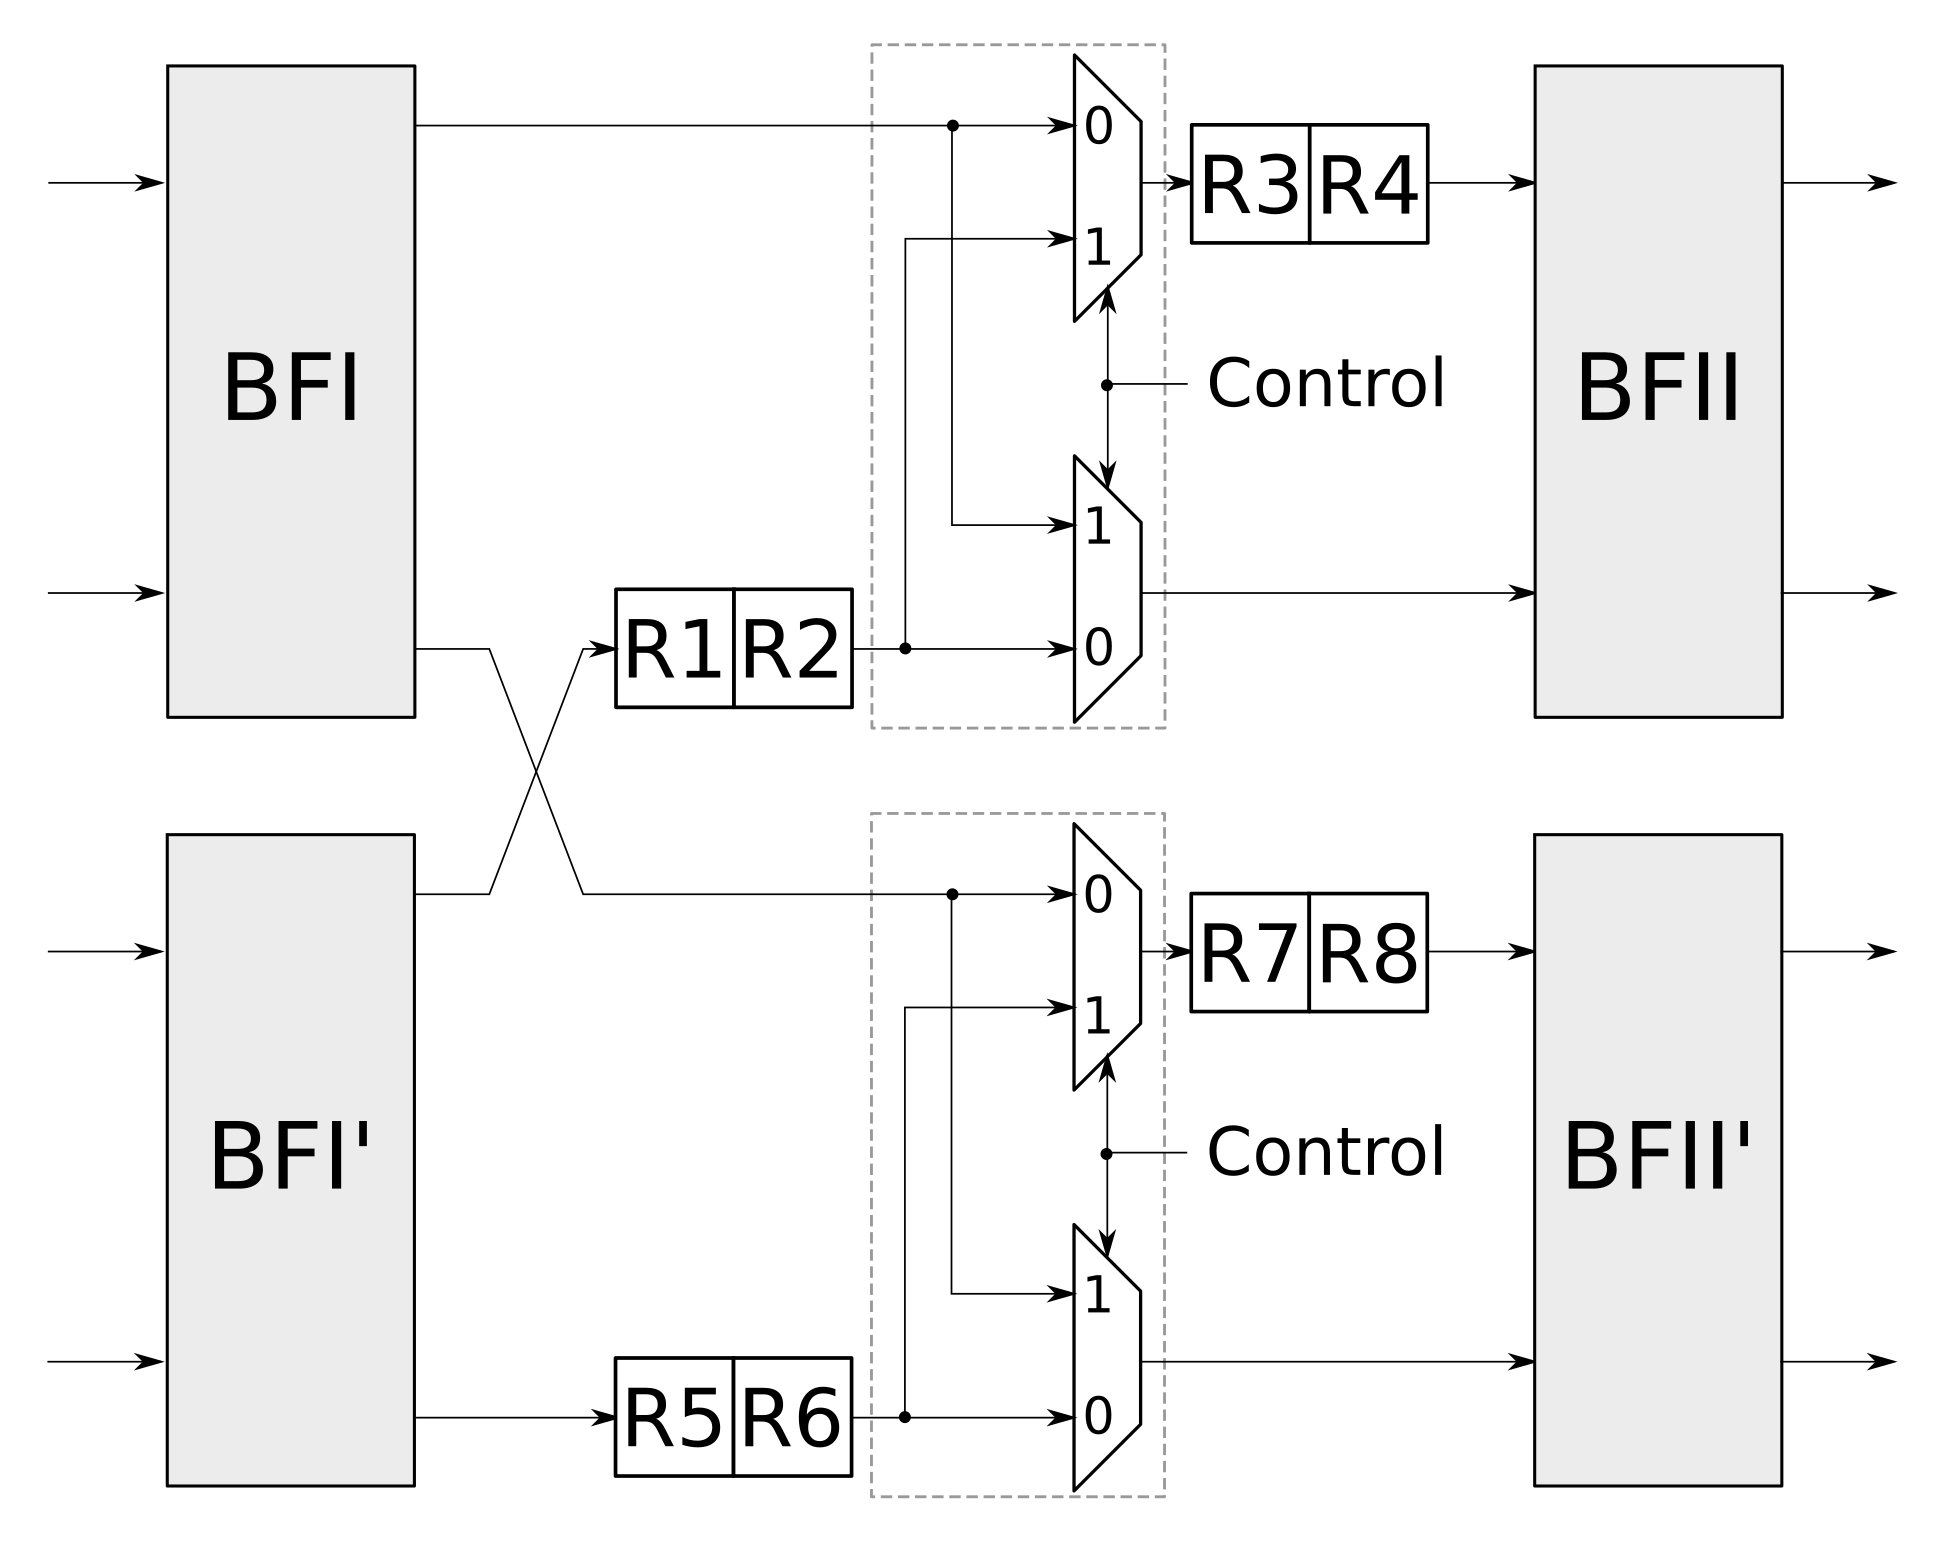
\includegraphics[width=0.85\linewidth]{Diagramas/folding_stage1.png}
        \caption{Registers names used in Fig. \ref{fig:tab-aloc-a} for stage 1.}
        \label{fig:folding16_stage1}
    \end{figure}
    %
  
    \begin{figure} 
        \centering
        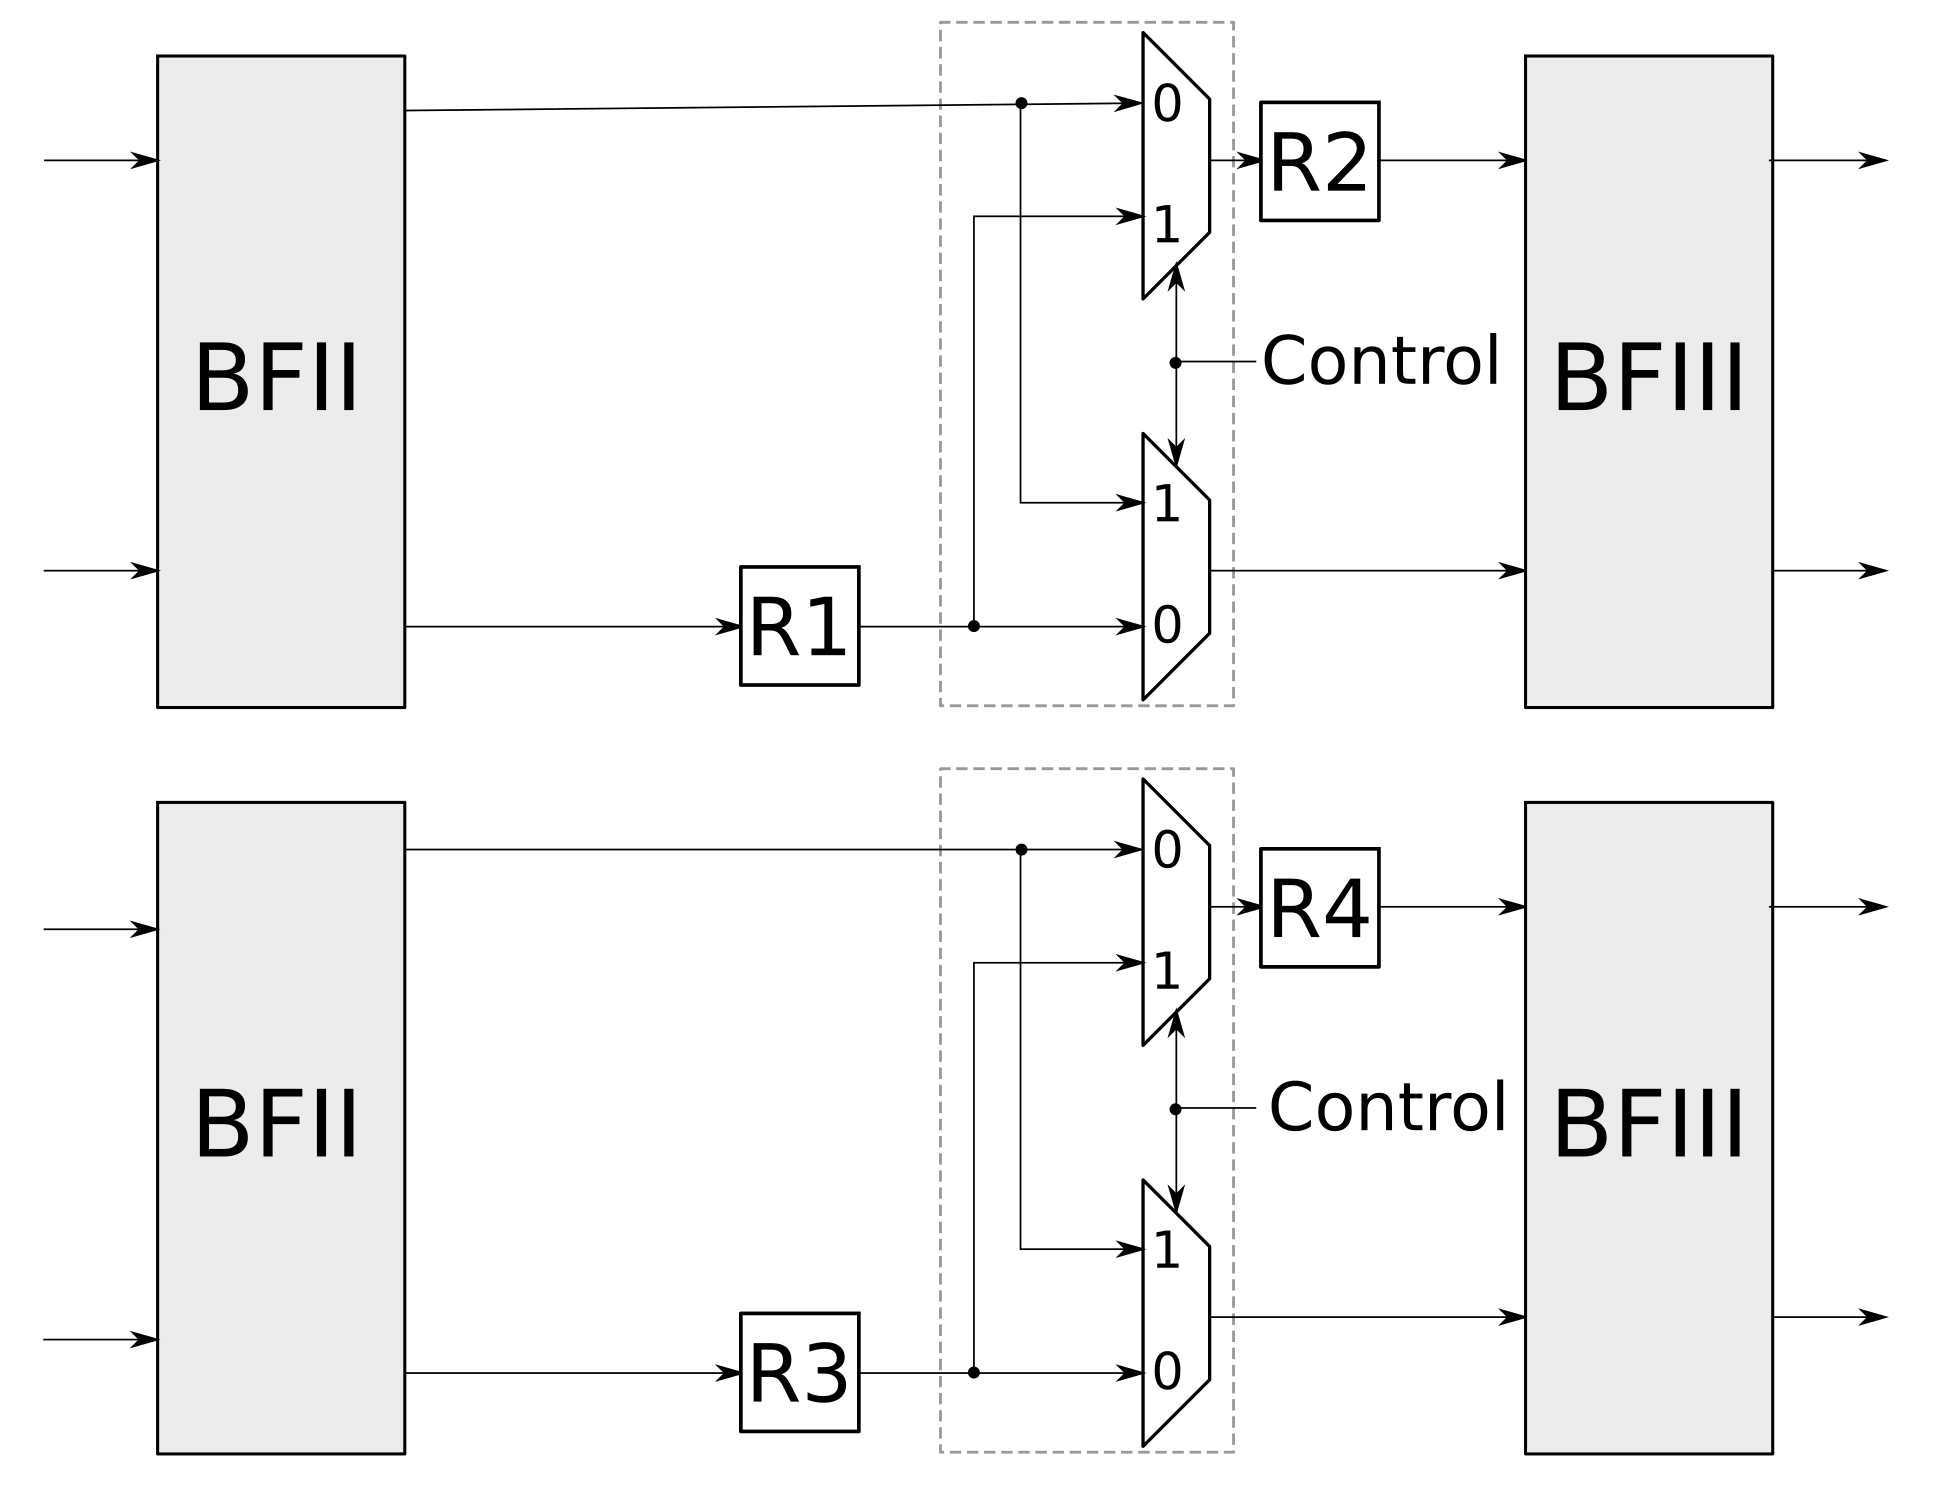
\includegraphics[width= 0.85\linewidth]{Diagramas/folding_stage2.png}
        \caption{Registers names used in Fig. \ref{fig:tab-aloc-b} for stage 2.}
        \label{fig:folding16_stage2}
    \end{figure}
        



As we can see in Fig. \ref{ fig:folding_16_arch}, we suppose that the inputs and output are not ordered, to order these variables extra logic are needed, using more registers and multiplexers.

The different types of rotators used in Fig. \ref{ fig:folding_16_arch} are shown in Fig. \ref{fig:rotators}, the description of each of them can be found below.
\begin{itemize}
	\item Trivial rotator: They can be carried out by interchanging the real and imaginary components and/or changing the sign of the data.
	\item Constant CSD rotator: They can be carried out by interchanging the real and imaginary components and a multiplication by a unique constant fractional number, in this case we will use a CSD multiplier to perform the area utilized.
	\item General rotator: They can be carried out by interchanging the real and imaginary components and/or a multiplication by more than one constant fractional numbers, in this case we will use a general multiplier.
\end{itemize}

\begin{figure} 
	\centering
	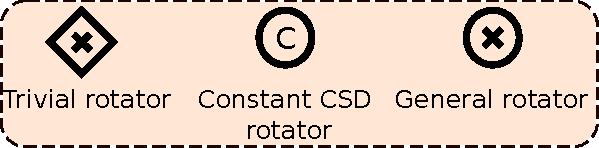
\includegraphics[width=0.6\linewidth]{Diagramas/miSeccionFiguras/Rotadores.pdf}
	\caption{Symbols used for the different types of rotators}
	\label{fig:rotators}
\end{figure}


\begin{figure*} 
	\centering
	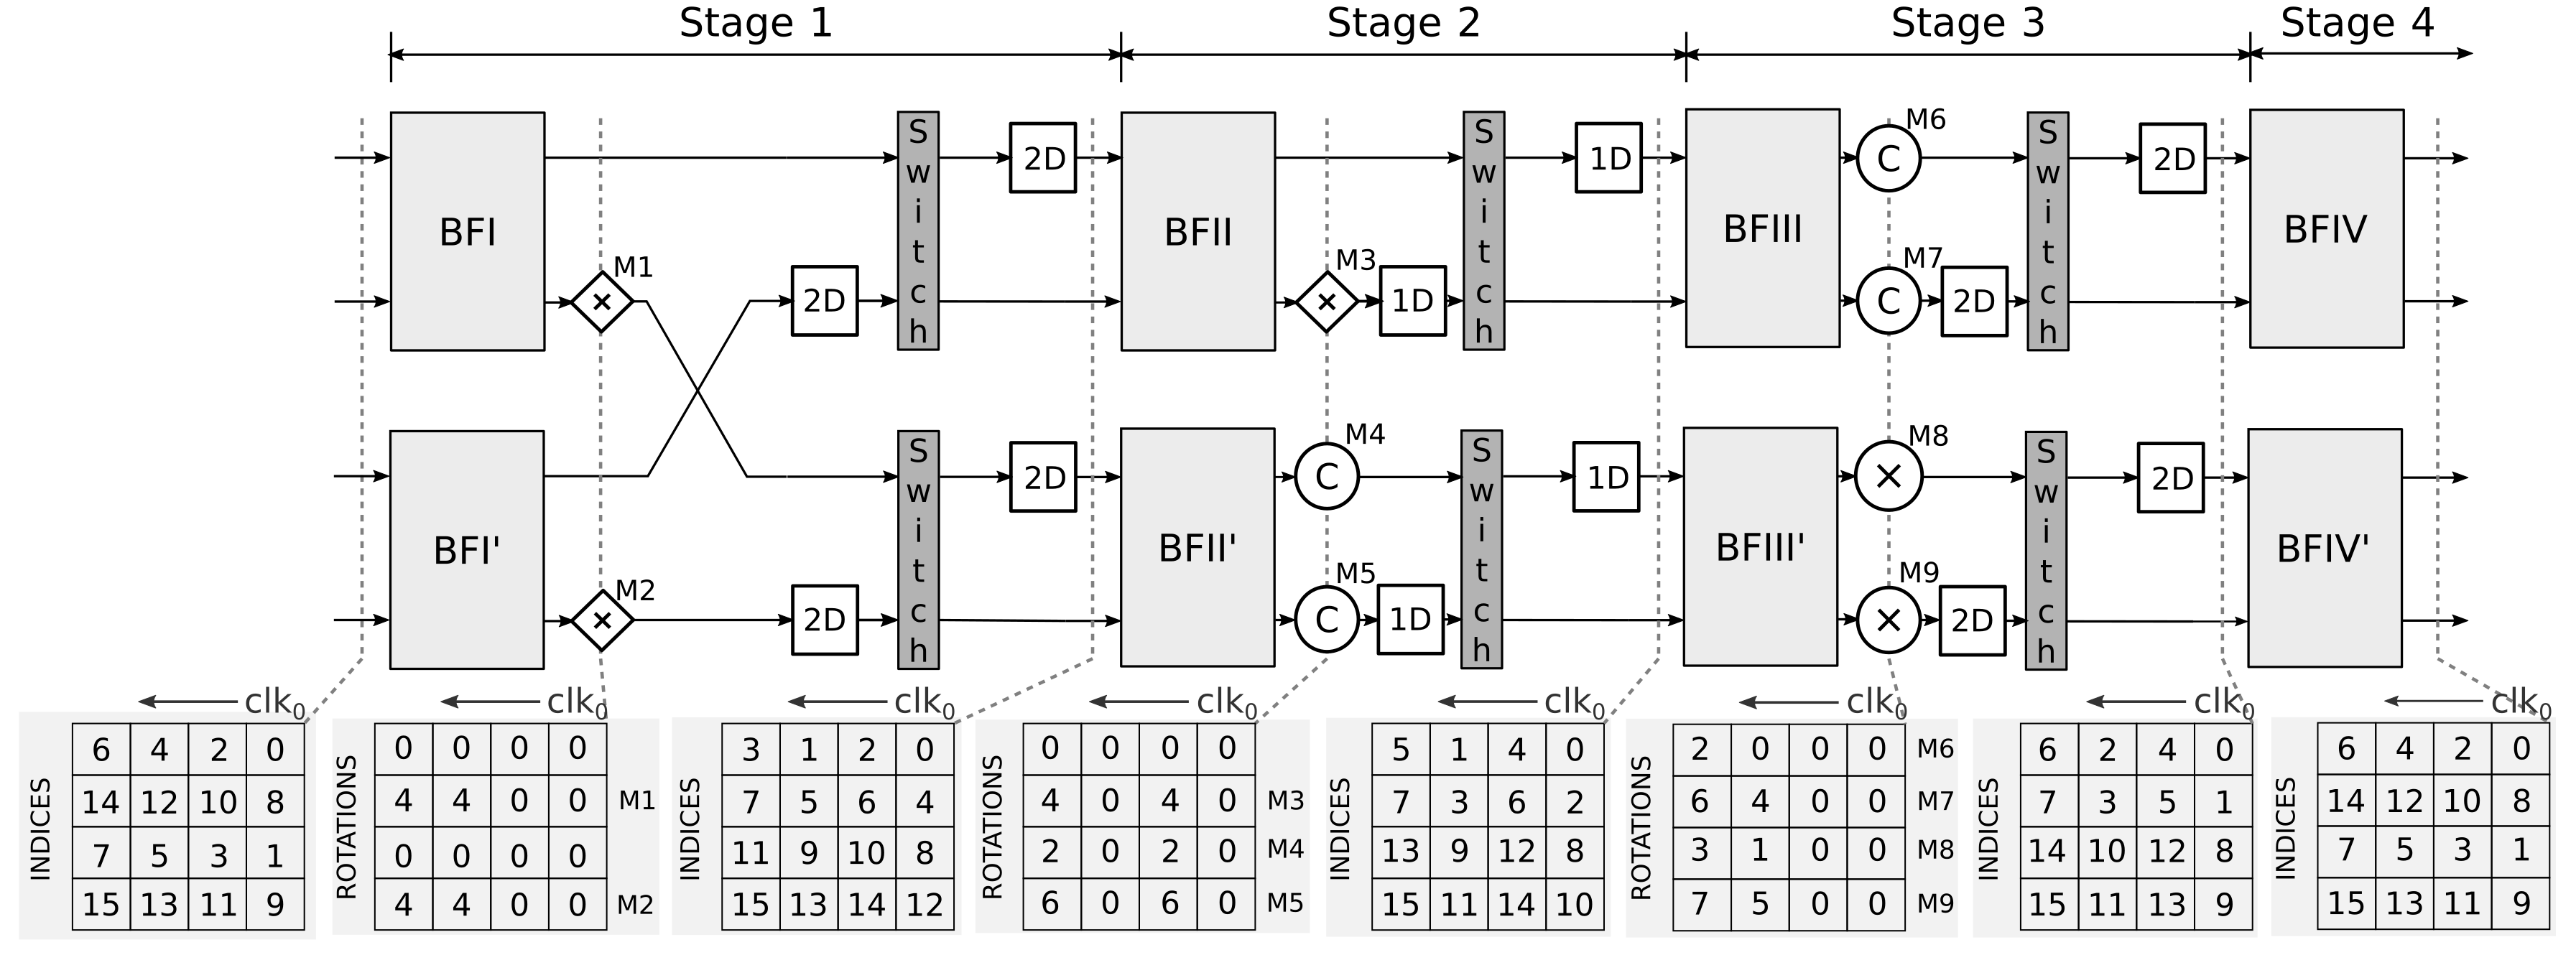
\includegraphics[width=\linewidth]{Diagramas/folding-16.png}
	\caption{Folding architecture for the computation of a radix-$2^3$ 16-point DIF complex FFT.}
	\label{fig:folding_16_arch}
\end{figure*}



%%%%%%%%%%%%%
%% Subseccion
%%%%%%%%%%%%%
\section{4-Parallel radix-$2^3$ 128-Points}   \label{sec:imp128}
We can deduce the folding architecture for 128 points following the same method than used with the 4-Parallel radix-$2^3$ 16-Points. The DFG and folding set used can be shown in Fig. \ref{fig:pipe_dfg_128} and Table \ref{tab:fold_set_128}.
The architecture can be seen in Fig. \ref{fig:circ-folding-128}.

%% Tabla de folding
\begin{small}
\begin{table*} 
	\centering
	\begin{threeparttable}
		\centering
		\caption{Folding set for the DFG showed in Fig. \ref{fig:pipe_dfg_128}}
		\label{tab:fold_set_128} 
		\begin{tabular}{|c||cccccccccccccccc|}
			\hline
			\multirow{2}{*}{A} & A0 & A2 & A4 & A6 & A8 & A10 & A12 & A14 & A16 & A18 & A20 & A22 & A24 & A26 & A28 & A30 \\  
			& A32 & A34 & A36 & A38 & A40 & A42 & A44 & A46 & A48 & A50 & A52 & A54 & A56 & A58 & A60 & A62 \\  
			\hline
			\multirow{2}{*}{A'} & A1 & A3 & A5 & A7 & A9 & A11 & A13 & A15 & A17 & A19 & A21 & A23 & A25 & A27 & A29 & A31 \\  
			& A33 & A35 & A37 & A39 & A41 & A43 & A45 & A47 & A49 & A51 & A53 & A55 & A57 & A59 & A61 & A63 \\  
			\hline
			\multirow{2}{*}{B} & B1 & B3 & B5 & B7 & B9 & B11 & B13 & B15 & B17 & B19 & B21 & B23 & B25 & B27 & B29 & B31 \\  
			& B0 & B2 & B4 & B6 & B8 & B10 & B12 & B14 & B16 & B18 & B20 & B22 & B24 & B26 & B28 & B30 \\  
			\hline
			\multirow{2}{*}{B'} & B33 & B35 & B37 & B39 & B41 & B43 & B45 & B47 & B49 & B51 & B53 & B55 & B57 & B59 & B61 & B63 \\  
			& B32 & B34 & B36 & B38 & B40 & B42 & B44 & B46 & B48 & B50 & B52 & B54 & B56 & B58 & B60 & B62 \\  
			\hline
			\multirow{2}{*}{C} & C16 & C18 & C20 & C22 & C24 & C26 & C28 & C30 & C1 & C3 & C5 & C7 & C9 & C11 & C13 & C15 \\  
			& C17 & C19 & C21 & C23 & C25 & C27 & C29 & C31 & C0 & C2 & C4 & C6 & C8 & C10 & C12 & C14 \\  
			\hline
			\multirow{2}{*}{C'} & C48 & C50 & C52 & C54 & C56 & C58 & C60 & C62 & C33 & C35 & C37 & C39 & C41 & C43 & C45 & C47 \\  
			& C49 & C51 & C53 & C55 & C57 & C59 & C61 & C63 & C32 & C34 & C36 & C38 & C40 & C42 & C44 & C46 \\  
			\hline
			\multirow{2}{*}{D} & D8 & D10 & D12 & D14 & D16 & D18 & D20 & D22 & D24 & D26 & D28 & D30 & D1 & D3 & D5 & D7 \\  
			& D9 & D11 & D13 & D15 & D17 & D19 & D21 & D23 & D25 & D27 & D29 & D31 & D0 & D2 & D4 & D6 \\  
			\hline
			\multirow{2}{*}{D'} & D40 & D42 & D44 & D46 & D48 & D50 & D52 & D54 & D56 & D58 & D60 & D62 & D33 & D35 & D37 & D39 \\  
			& D41 & D43 & D45 & D47 & D49 & D51 & D53 & D55 & D57 & D59 & D61 & D63 & D32 & D34 & D36 & D38 \\  
			\hline
			\multirow{2}{*}{E} & E4 & E6 & E8 & E10 & E12 & E14 & E16 & E18 & E20 & E22 & E24 & E26 & E28 & E30 & E1 & E3 \\  
			& E5 & E7 & E9 & E11 & E13 & E15 & E17 & E19 & E21 & E23 & E25 & E27 & E29 & E31 & E0 & E2 \\  
			\hline
			\multirow{2}{*}{E'} & E36 & E38 & E40 & E42 & E44 & E46 & E48 & E50 & E52 & E54 & E56 & E58 & E60 & E62 & E33 & E35 \\  
			& E37 & E39 & E41 & E43 & E45 & E47 & E49 & E51 & E53 & E55 & E57 & E59 & E61 & E63 & E32 & E34 \\  
			\hline
			\multirow{2}{*}{F} & F2 & F4 & F6 & F8 & F10 & F12 & F14 & F16 & F18 & F20 & F22 & F24 & F26 & F28 & F30 & F1 \\  
			& F3 & F5 & F7 & F9 & F11 & F13 & F15 & F17 & F19 & F21 & F23 & F25 & F27 & F29 & F31 & F0 \\  
			\hline
			\multirow{2}{*}{F'} & F34 & F36 & F38 & F40 & F42 & F44 & F46 & F48 & F50 & F52 & F54 & F56 & F58 & F60 & F62 & F33 \\  
			& F35 & F37 & F39 & F41 & F43 & F45 & F47 & F49 & F51 & F53 & F55 & F57 & F59 & F61 & F63 & F32 \\  
			\hline
			\multirow{2}{*}{G} & G3 & G5 & G7 & G9 & G11 & G13 & G15 & G17 & G19 & G21 & G23 & G25 & G27 & G29 & G31 & G0 \\  
			& G2 & G4 & G6 & G8 & G10 & G12 & G14 & G16 & G18 & G20 & G22 & G24 & G26 & G28 & G30 & G1 \\  
			\hline
			\multirow{2}{*}{G'} & G35 & G37 & G39 & G41 & G43 & G45 & G47 & G49 & G51 & G53 & G55 & G57 & G59 & G61 & G63 & G32 \\  
			& G34 & G36 & G38 & G40 & G42 & G44 & G46 & G48 & G50 & G52 & G54 & G56 & G58 & G60 & G62 & G33 \\
			\hline
		\end{tabular}
	\end{threeparttable}
\end{table*}
\end{small}

\begin{figure*} 
	\centering
	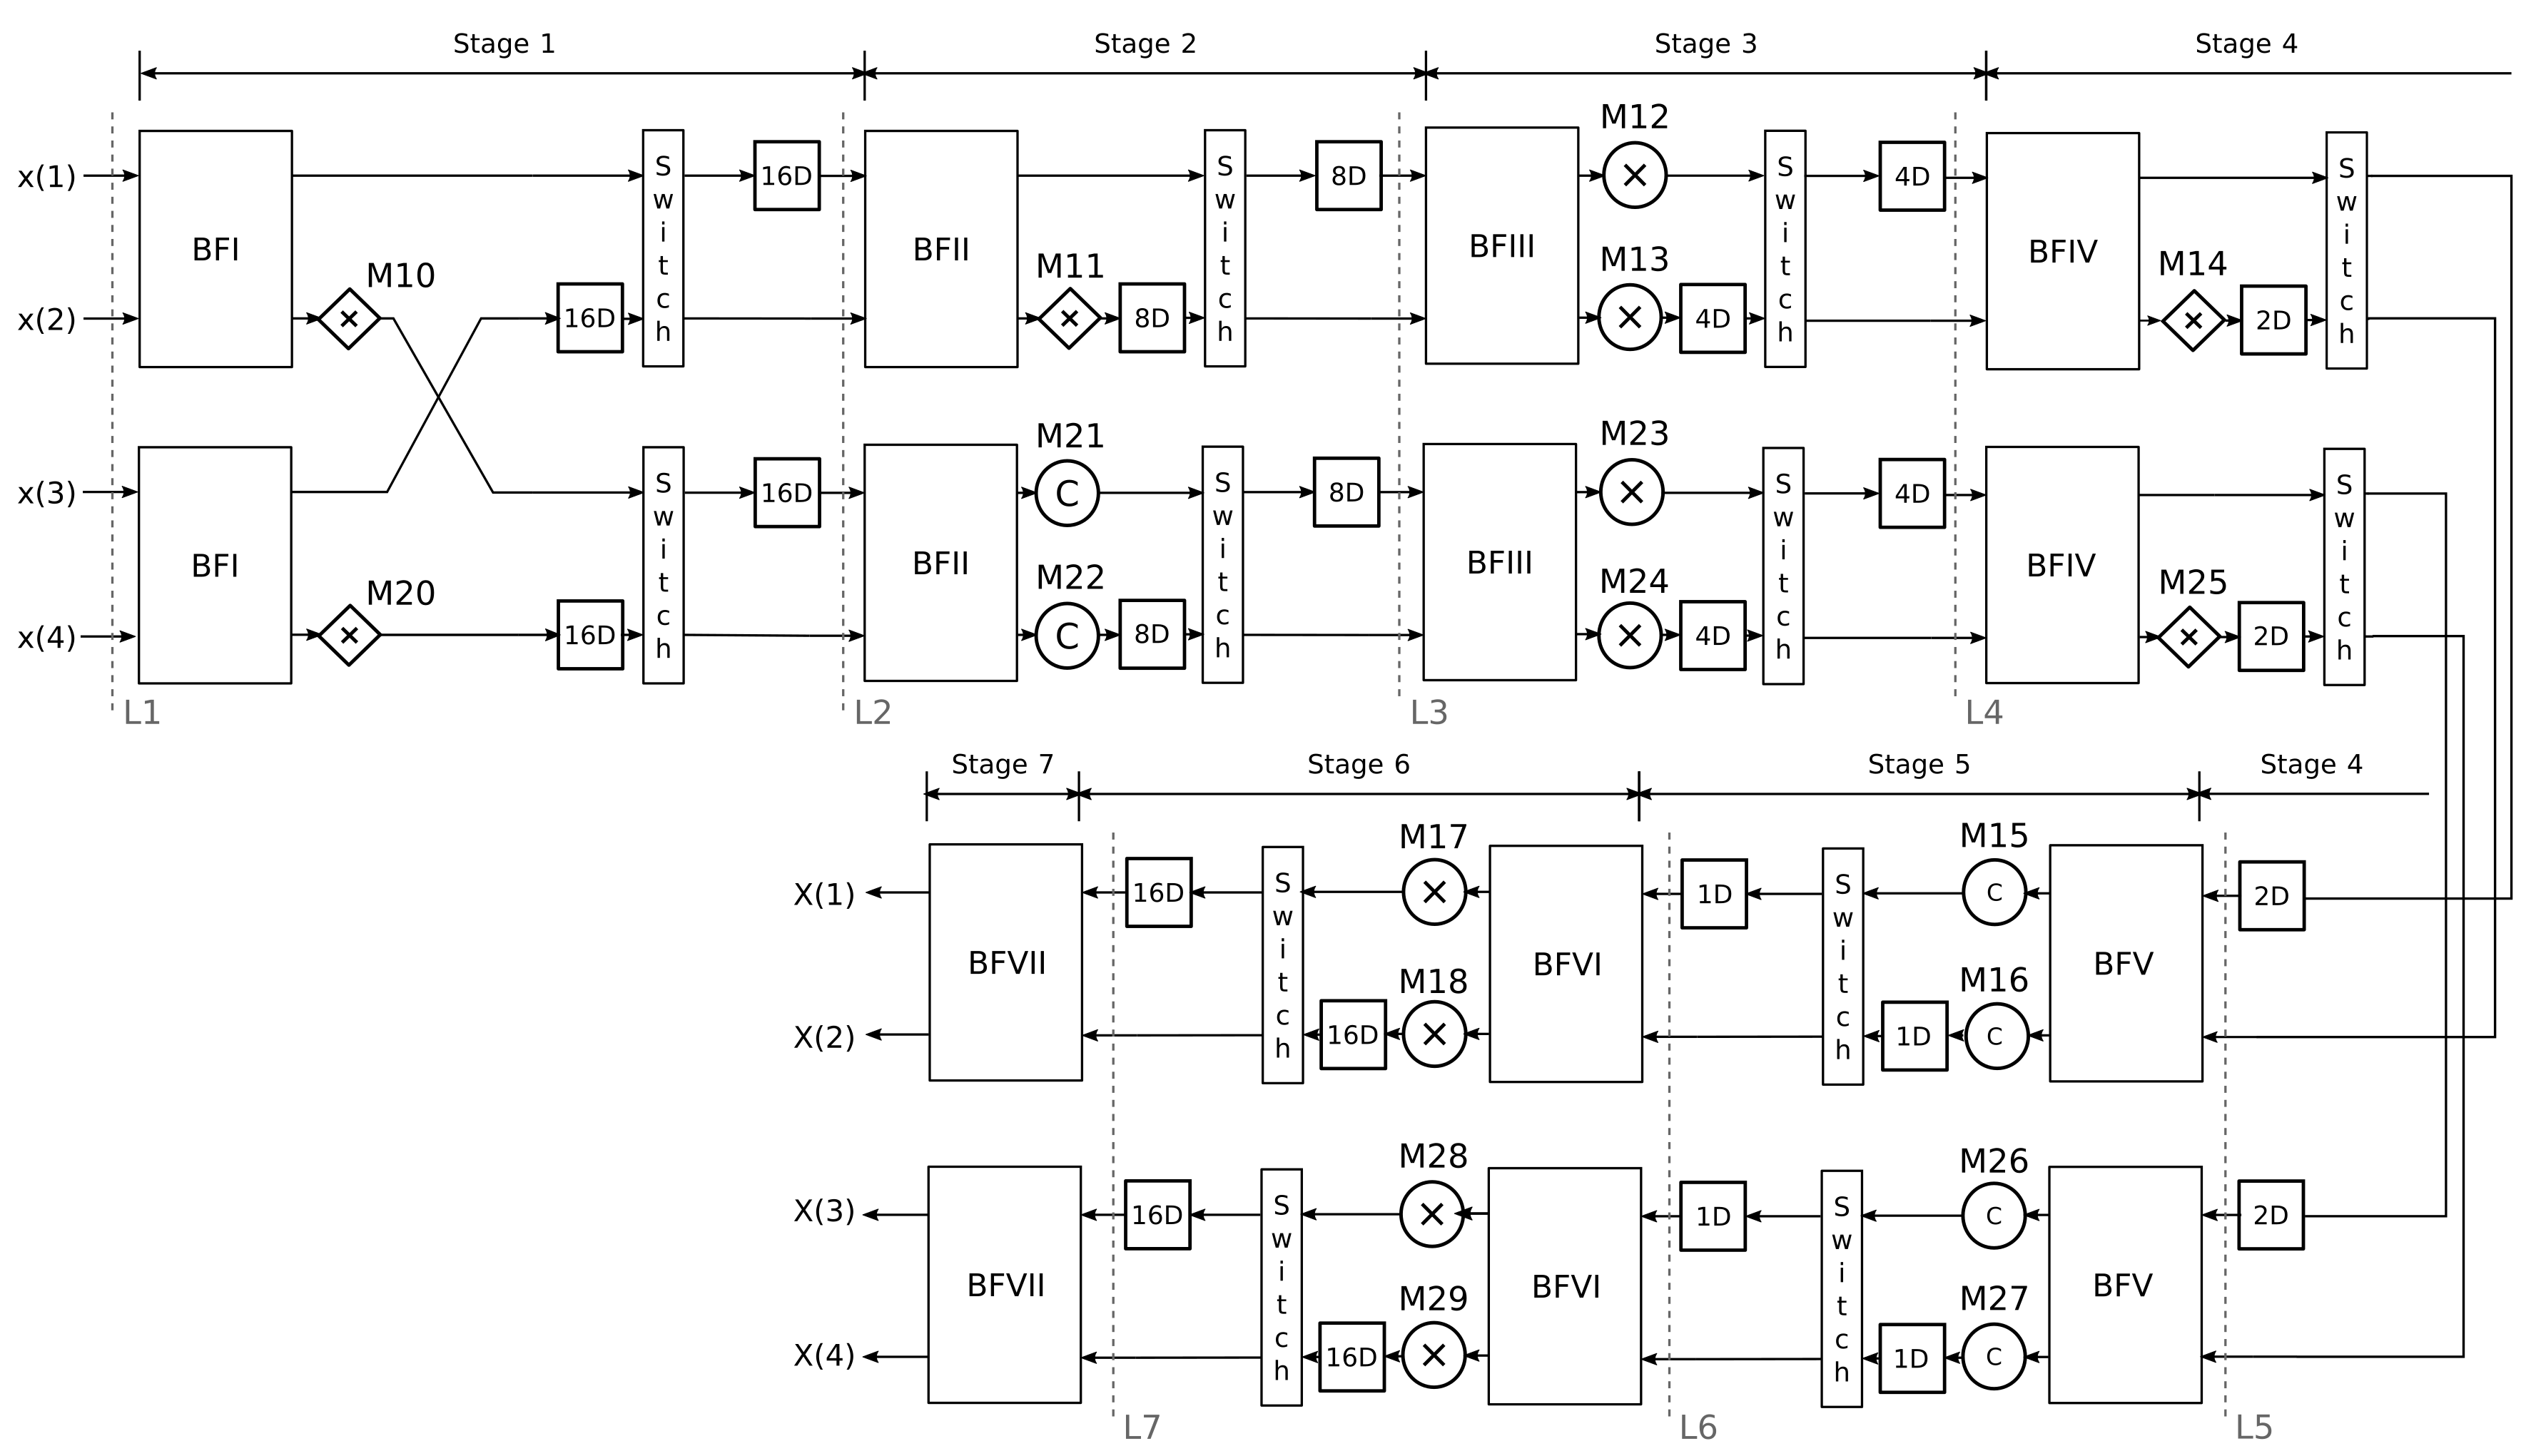
\includegraphics[width=0.8\linewidth]{Diagramas/folding-128.png}
	\caption{Folding architecture for the computation of a radix-$2^3$ 128-point DIF complex FFT.}
	\label{fig:folding_128}
\end{figure*}



%%%%%%%%%%
%% Seccion
%%%%%%%%%%
 
\subsection{Implementation of a 128-point FFT}
In this section we are going to begin with the process of how accomplish the implementation of our 4-parallel architecture for the computation of 128-point \textit{radix}-$2^3$ DIF complex FFT.
First, we wrote a \textit{MATLAB} simulator to validate the operation of our design and the design presented in \cite{garrido_pipelined_2013,garrido_feedforward_2018}. Therefore, we can have a reference architecture for compare the design that we deduce. After that, we take all these information to generate a Synthesizable \textit{Verilog} code with different levels of optimizations with a powerful tool like \textit{Synopsys} to get a final design integrated of Standard Cells $@45nm$.
%%%%%%%%%%%%%
%% Subseccion
%%%%%%%%%%%%%
\subsection{Floating and Fixed point Simulator}
\begin{figure*} 
	\centering
	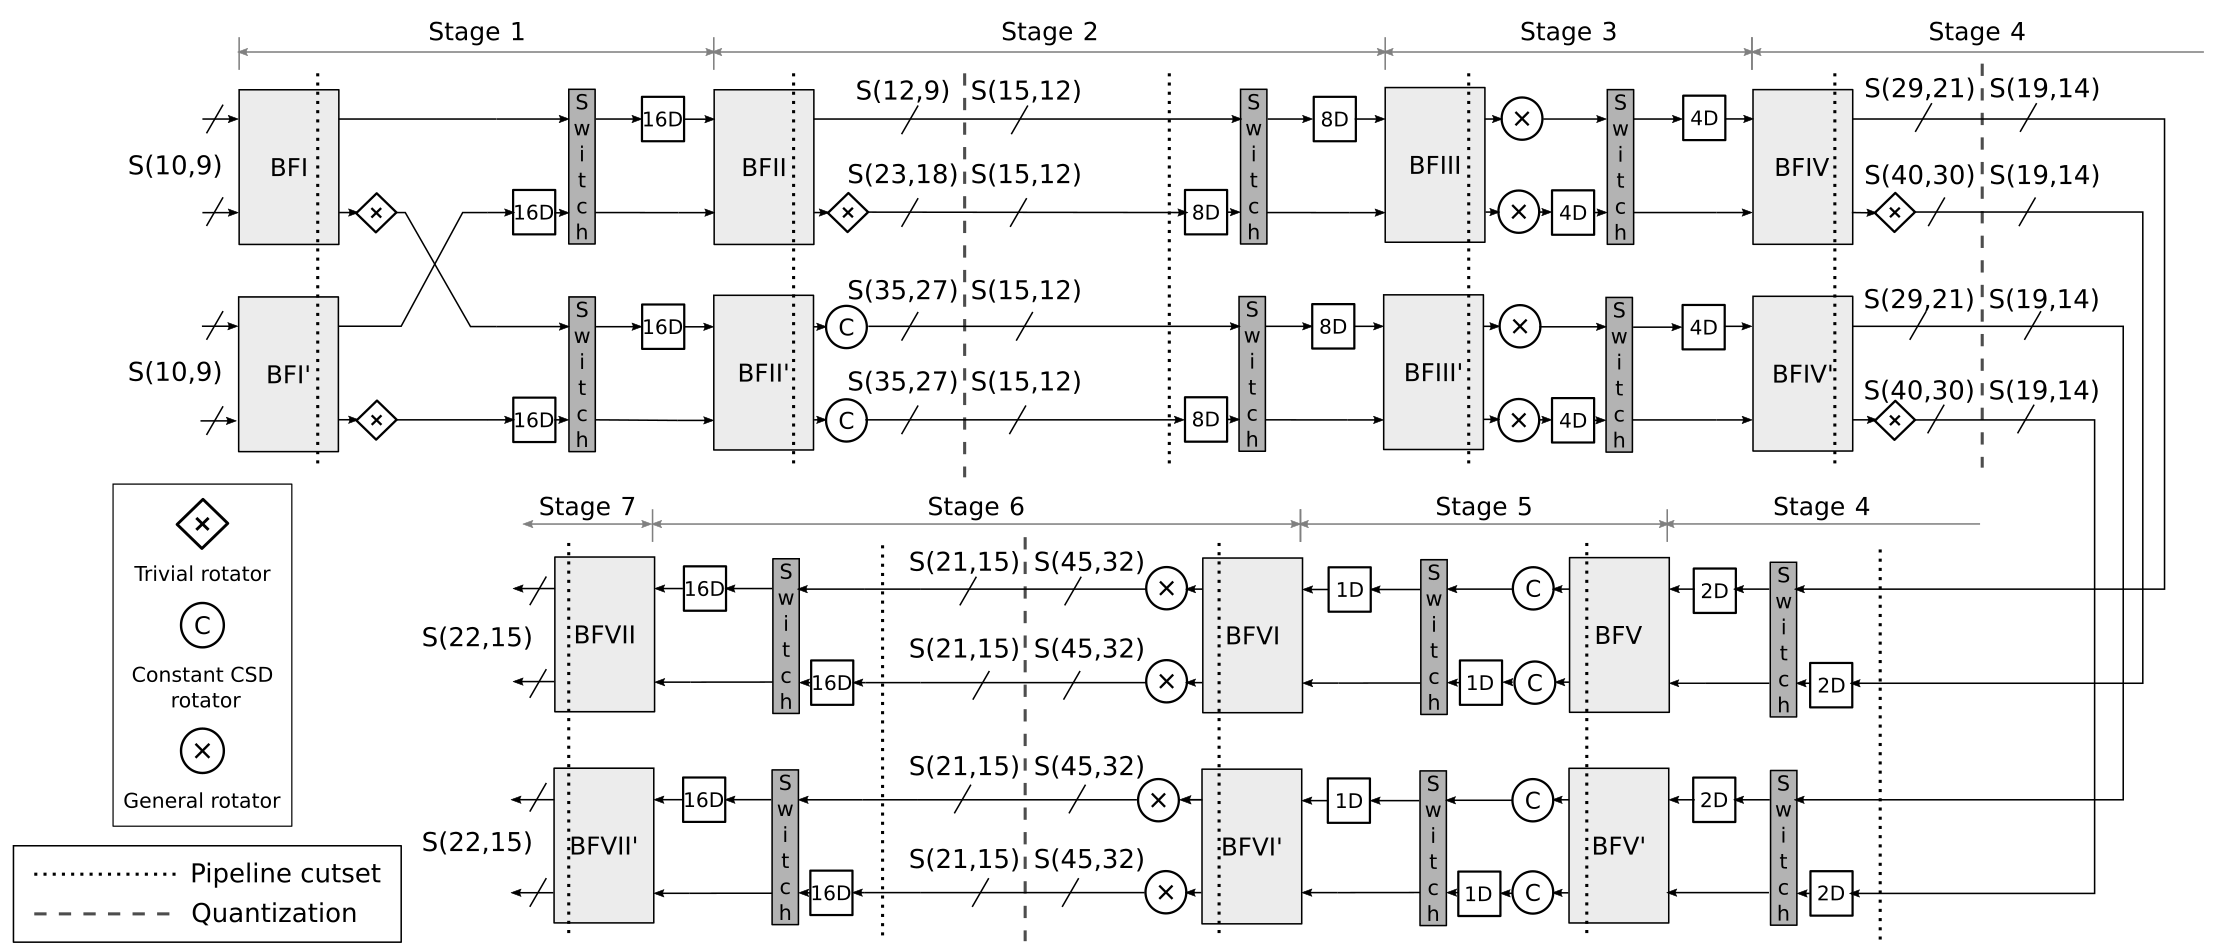
\includegraphics[width=0.95\linewidth]{Diagramas/folding-128-quant-pipe.png}
	\caption{Quantization for a 128-point 4-parallel complex FFT architecture}
	\label{fig:4paralelo128pradix8cuantizacion1}
\end{figure*}


\begin{figure} 
	\centering
	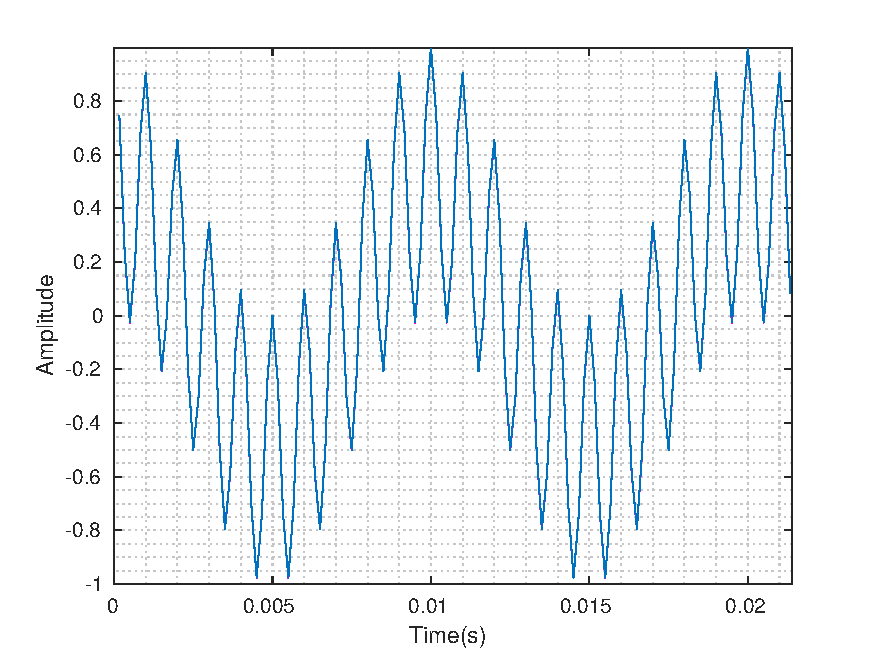
\includegraphics[width=0.92\linewidth]{Diagramas/DftInputSignal.pdf}
	\caption{Input signal $x[n]$ in time domain}
	\label{fig:dftinputsignal}
\end{figure}

\begin{figure} 
	\centering
	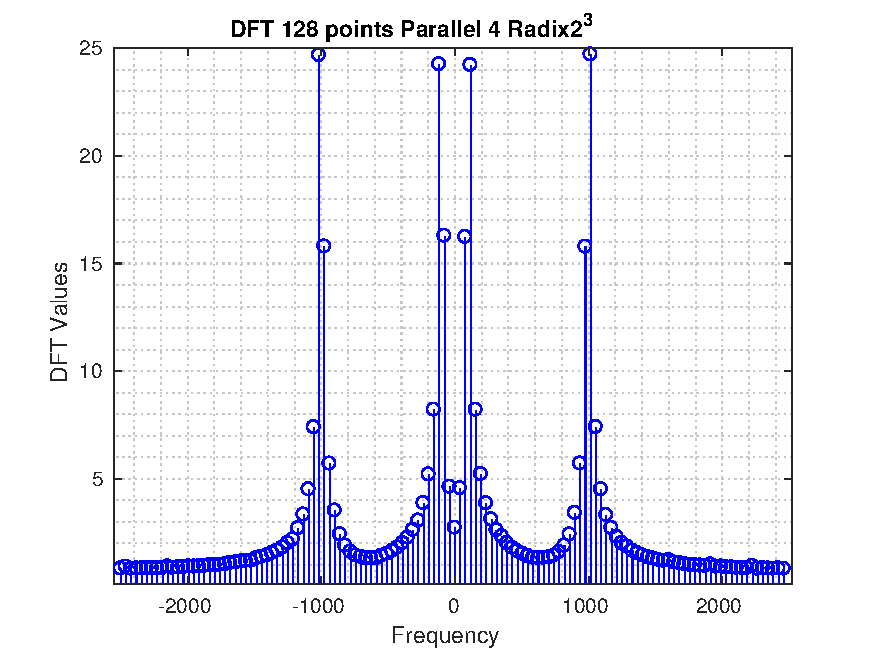
\includegraphics[width=0.95\linewidth]{Diagramas/DftFixedPoint.pdf}
	\caption{Output samples, absolute value vs frequency $|X[k]|$}
	\label{fig:dftfixedpoint}
\end{figure}
The input signal Fig. \ref{fig:dftinputsignal} to our architecture will be a mixture of sinusoid signals with two frequency values, theses signal will be normalizing to the unity and in this way we can have a test bench design.
\begin{align}\label{eq: inputSignal}
x'[n] &= cos(2\pi f_1 n T_s) + cos(2\pi f_2 n T_s)  \\
x[n] &= x'[n]/max\{x'[n]\} 						\nonumber
\end{align}
where $f_1=100Hz$, $f_2=1000Hz$ and $T_s$ is the sampled period.

In each stage of the Fig. \ref{fig:4paralelo128pradix8cuantizacion1}, input samples that propagate stage by stage will be carefully quantized with the purpose of getting a high SQNR (Signal to Quantization Noise Ratio).
\begin{equation*}%\label{eq:sqnr}
SQNR_{dB} = 10log_{10} \bigg(  \frac{  Var\{Signal_{FloatPoint}\}  }{  Var\{Signal_{FloatPoint} - Signal_{FixedPoint}\}}  \bigg)
\end{equation*}
SQNR computation represents the logarithmic relationship between float signal variance over error variance from an signal given.

The input signal $x[n]$ is quantized with a value of $S(10,9)$, that representation means a number signed (S) with $10$ total bits and $9$ fractional bits. The value calculated of SQNR for the input is $56.9dB$. Following the same steps, we can compute the SQNR for the \textit{twiddle} factors and the architecture's output.

Twiddles factor are quantized with a relation of $S(11,9)$ and the complex output signal $X[k]$ with $S(22,15)$. Output quantization for the real part is $46.8dB$ and for the imaginary part $47.3dB$. In general, a value of quantization close to $50dB$ is a good approximation. Out signal from our \textit{MATLAB} fixed-point model from the architecture in Fig. \ref{fig:4paralelo128pradix8cuantizacion1} the output signal is given in Fig. \ref{fig:dftfixedpoint}, that represents a first approach in our calculation of a DFT without optimization.

\begin{figure} 
	\centering
	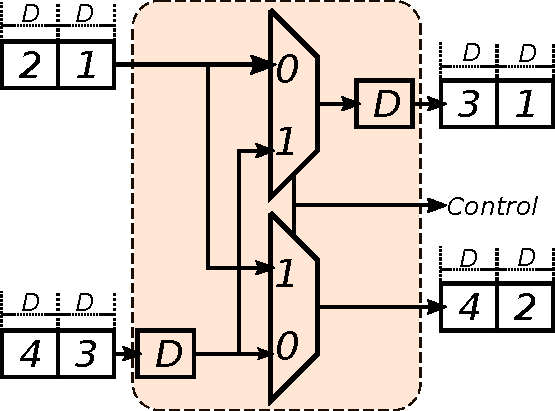
\includegraphics[width=0.42\linewidth]{Diagramas/miSeccionFiguras/Shift.pdf}
	\caption{Circuit for data shuffling}
	\label{fig:shift}
\end{figure}
\begin{figure} 
	\centering
	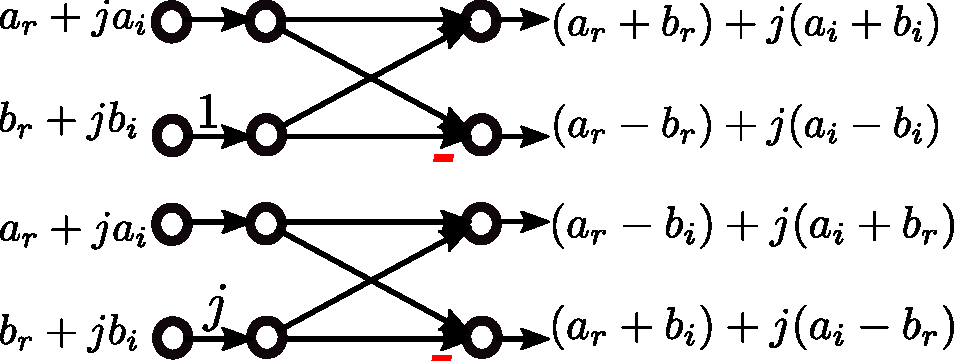
\includegraphics[width=0.65\linewidth]{Diagramas/miSeccionFiguras/ButterComplejo.pdf}
	\caption{Complex butterfly }
	\label{fig:buttercomplejo}
\end{figure}
\begin{figure} 
	\centering
	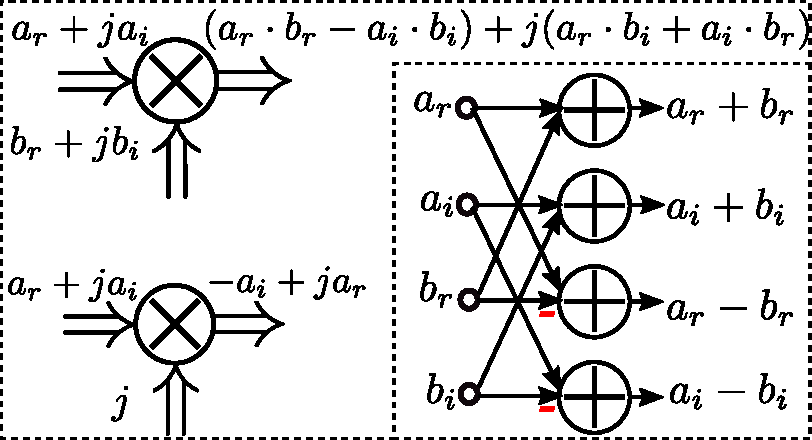
\includegraphics[width=0.65\linewidth]{Diagramas/miSeccionFiguras/SumMult.pdf}
	\caption{Complex multiplier and complex adder}
	\label{fig:summult}
\end{figure}

The combination between latencies (delays registers) and switches in all stages in Fig. \ref{fig:4paralelo128pradix8cuantizacion1} is the equivalent circuit shows in Fig. \ref{fig:shift}, that is used to appropriately order samples in each butterflies input.

Whole elements on the architecture such as multipliers and butterflies are complex as Fig. \ref{fig:buttercomplejo} and \ref{fig:summult}. On an implementation is essential divide the signal in its real and imaginary part with the purpose of process them independently. A \textit{general rotator} (full complex multiplier) generate a real and imaginary component that is composed by a real multiplication an one addition, but a \textit{trivial rotator} only change the components of a complex signal. These relations are important at the moment of doing the quantization process to ensure an appropriate quantity of bits.
%%%%%%%%%%%%%
%% Subseccion
%%%%%%%%%%%%%
\subsection{Verilog (HDL) Model} 
%\begin{figure*} 
%	\centering
%	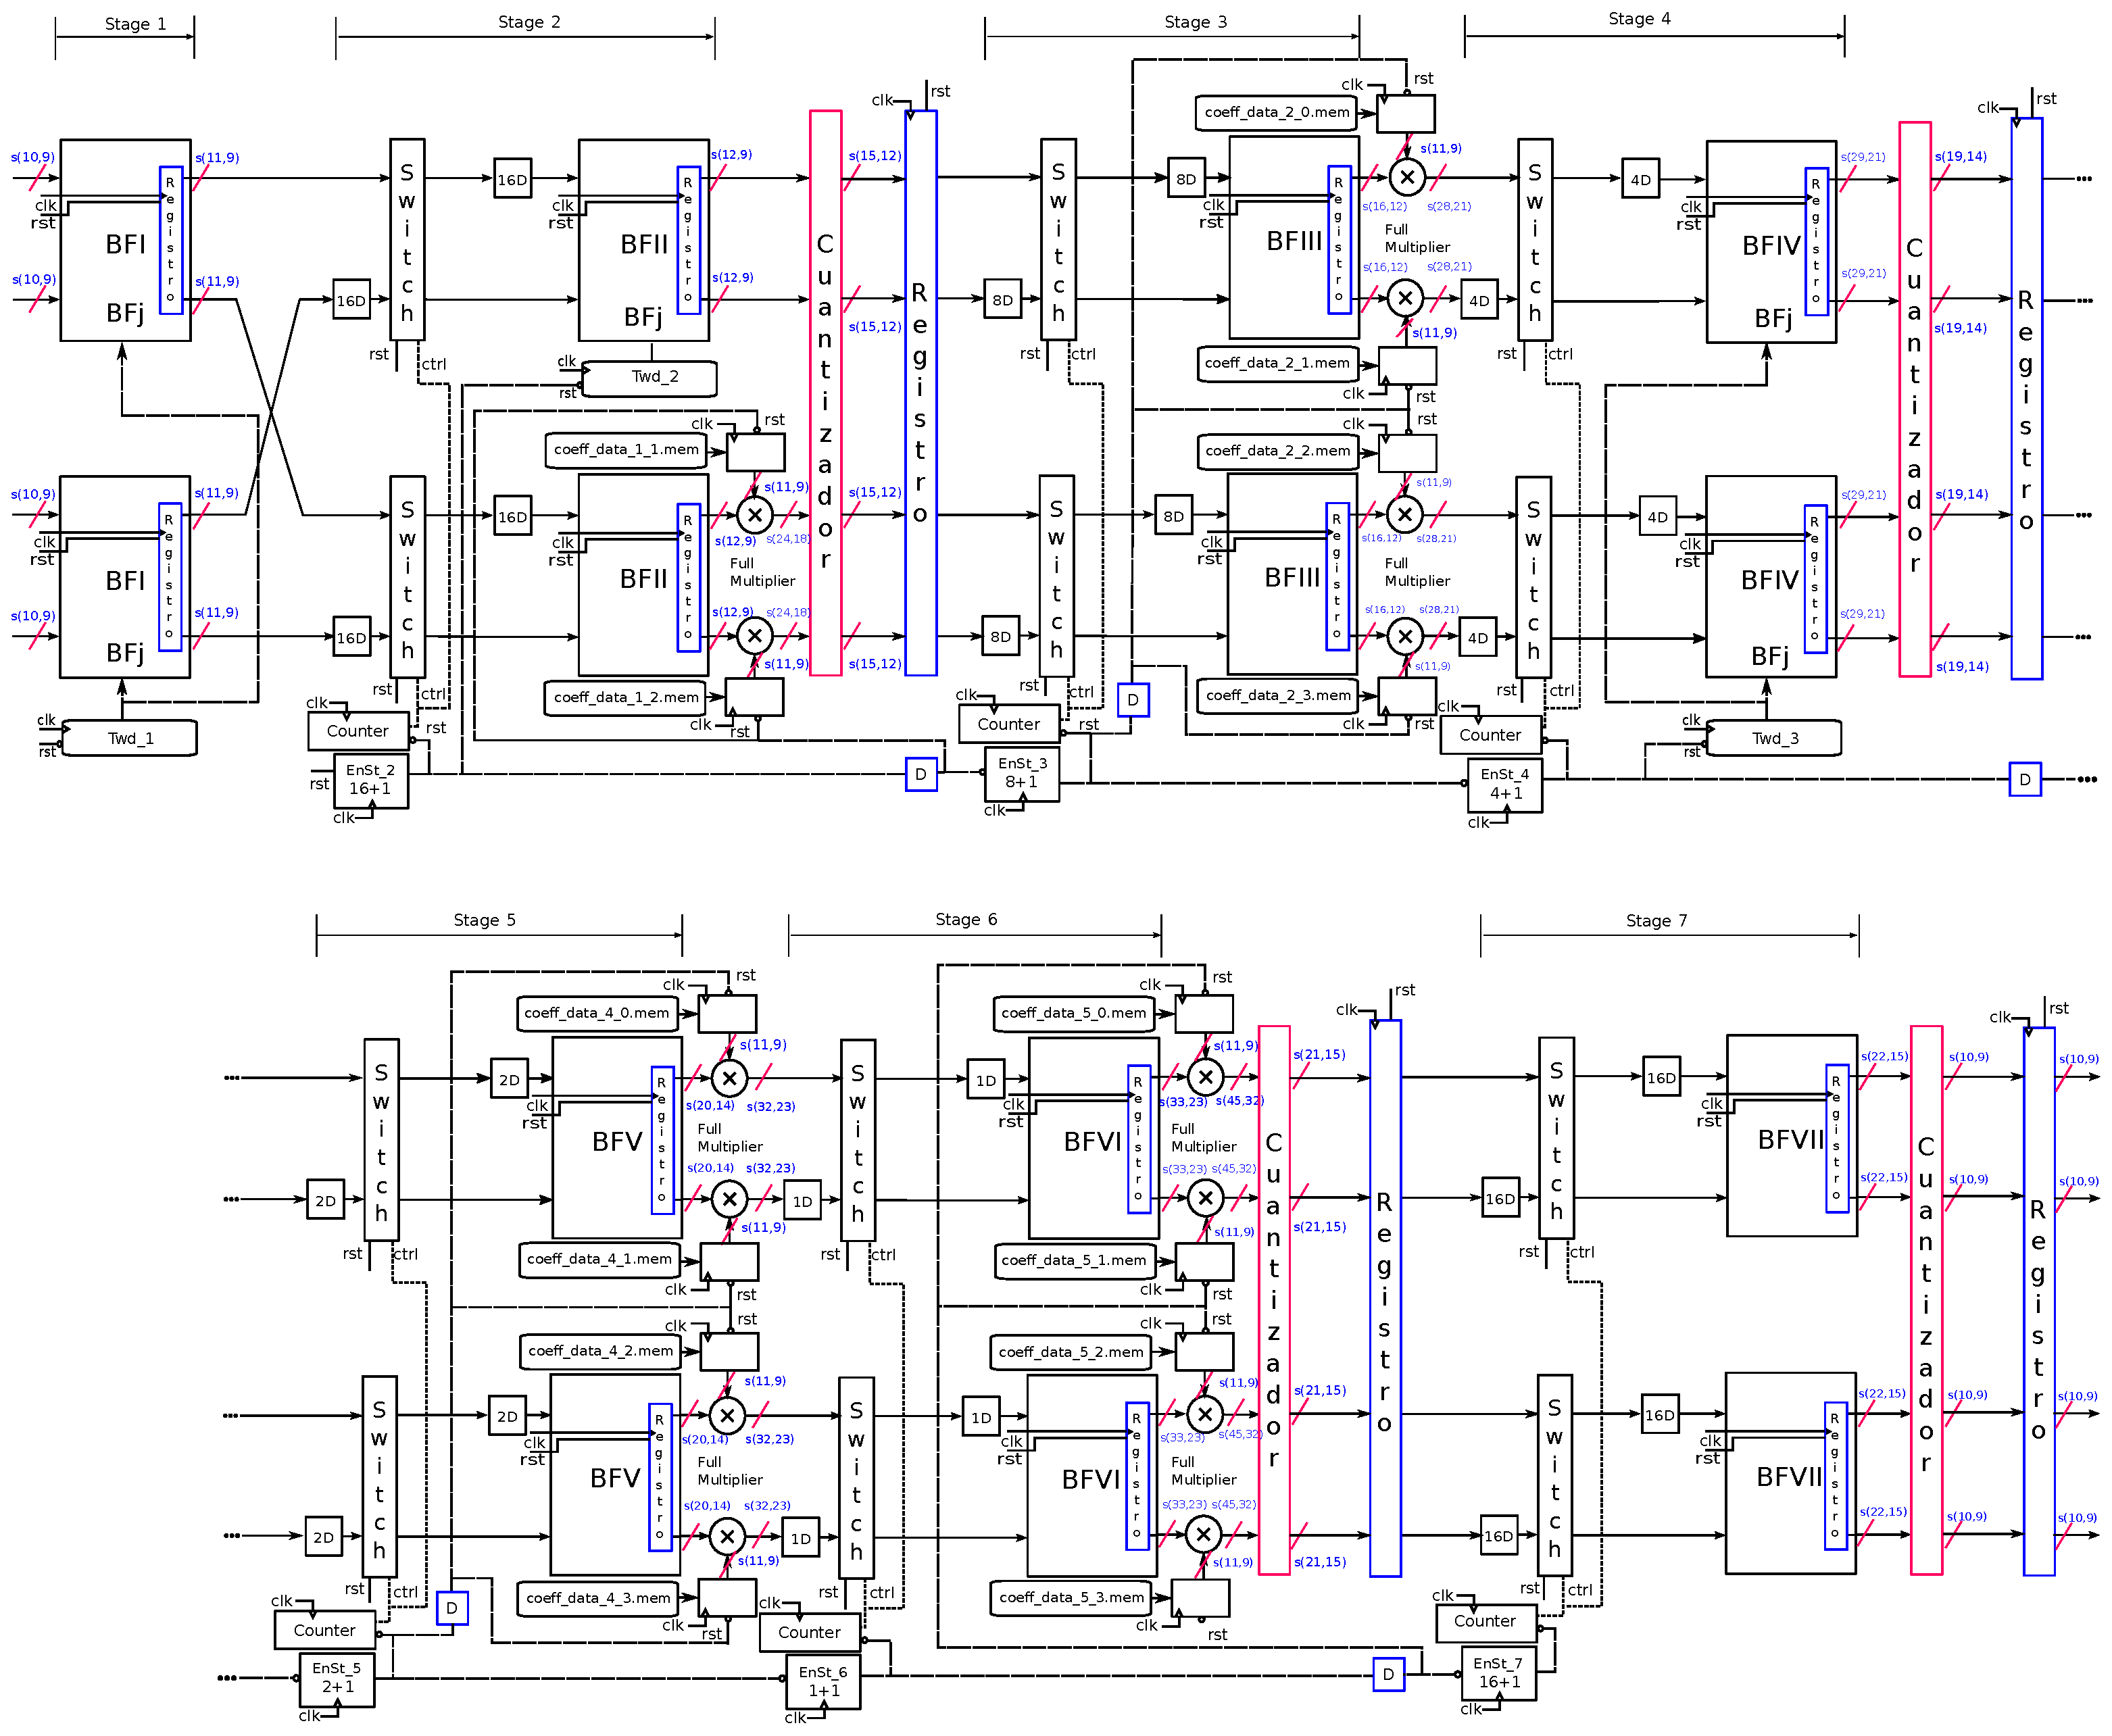
\includegraphics[width=\linewidth]{Diagramas/V5_esquema_p.eps}
%	\caption{RTL (Register transfer level) design for a 4-parallel \textit{radix}-$2^3$ 128-point DIF FFT with Optimization}
%	\label{fig:v5esquemap}
%\end{figure*}

In this subsection we are going to talk about the different design instances to model the DFT in hardware. 
We made four design implementations with the purpose of have a global view of optimization levels to achieve the requested \textit{Timing} at a working frequency of 500MHz obtained from the synthesis processes.

In the first instance of design was made from the base design showed in Fig. \ref{fig:4paralelo128pradix8cuantizacion1}, this hardware model has butterflies modules that work in combination with multipliers and each multiplier has associated a memory block that contains twiddle factors. In this first approach all multipliers are \textit{full}, each stage has a control module that enable and disable the inversion of the switching block, this control signal is also sent to the multipliers to work synchronously with the switching. To avoid the bit growth generated by the addition and multiplication, a quantization block is necessary, the quantizer consisted of saturation and truncate operations.

In the second place with the goal of minimize the \textit{critical path} in our design, we add \textit{pipelined} registers after quantization blocks. In the third case of implementation incorporate \textit{trivial} multipliers, imaginary multiplication by -$1j$, with this kind of operation we can reduce the size of the binary word. 

In the fourth level of optimization showed in Fig. \ref{fig:v5esquemap}, we place inside each butterfly blocks an internal pipelined to improve the required timing. Lastly, the full multipliers from stage two and five are modified to efficiently work with constant coefficients, these new multipliers are \textit{CSD} because the twiddle factors in these stages are always $-je^{-j\frac{\pi}{4}}$ and $e^{-j\frac{\pi}{4}}$.


%%%%%%%%%%
%% Seccion
%%%%%%%%%%
 
\section{Results}  \label{sec:results}
All designs were implemented with different levels of optimization to accomplish the desired working frequency. The design instances were synthesized by Synopsys tool in order to build an interconnection of Standard Cells to get and generate a complete set of \textit{timing-area-power report} showed in Table \ref{tab:reporte2}, \ref{tab:reporte5} and  \ref{tab:reporte6}. According to the first results, data arrival time is greater than minimum period established 2ns and we can detected that there is a time Violated, with this first approach we decide make a set of optimizations to folding architecture as a pipelined cutset between stages of DFT. In this way as we can see in Table \ref{tab:reporte5}, we reduced power, area and timing. 

In contrast with the first instance of design, we found in the last case of implementation a slack of time equal to zero, that means the clock period satisfy the time constraint at 500MHz.

%% primera version sin pipe y sin saturation, no llega a 500MHz
\begin{table}
	\centering%\raggedleft%\flushright
	\caption{Design instance 1. Timing-Area-Power Report at 500MHz}
	\label{tab:reporte2}
	\begin{tabular}{@{}lr@{}}
		%\hline\hline
		Point 						& Path(ns)\\
		\hline\hline
		data arrival time   		& 5.60\\ 
		clock CLK (rise edge)  		& 2.00\\
		clock network delay (ideal) & 2.00\\
		library setup time			& 1.95\\
		\hline
		data required time			& 1.95\\
		data arrival time           & -5.60\\
		\hline
		slack (VIOLATED)            & -3.65\\	
		\hline
	\end{tabular}

	\begin{tabular}{@{}lr@{}}\\
		Logical Elements\\
		\hline\hline
		Number of ports               &1228\\
		Number of nets                &112376\\
		Number of cells               &102726\\
		Number of combinational cells &95310\\
		Number of sequential cells    &7404\\
		Number of macros/black boxes  &0\\
		Number of buf/inv             &27817\\
		\hline
		Combinational area            &291201.116637\\
		Buf/Inv area                  &44892.767764\\
		Noncombinational area         &58830.508095\\
		\hline
		Total cell area               &350031.624731\\	
		\hline
	\end{tabular}

	\begin{tabular}{@{}lcccr@{}}\\
		Power Group		 &Internal 	&Switching 	&Leakage		&Total Power\\
		\hline\hline
		io pad           &0.0000    &0.0000     &0.0000    		&0.0000\\
		clock network    &34.8220   &603.2268   &1.4573e+06 	&639.6328\\
		register         &54.2228   &0.2699     &4.0540e+05 	&54.8980\\  
		sequential       &0.0000    &0.0000     &0.0000     	&0.0000\\  
		combinational    &0.2884    &0.7304     &1.5016e+04 	&1.0337\\ 
		\hline
		Total            &89.333mW  &604.227mW  &1.877e+06nW	&695.564mW\\	
		\hline
	\end{tabular}
%	\label{tab:rep_desgin1}
\end{table}
%\begin{table} 
	\centering%\raggedleft%\flushright
	\caption{Design instance 2. Timing-Area-Power Report at 500MHz}
	\label{tab:reporte3} 		
	\begin{tabular}{@{}lr@{}}
		%\hline\hline
		Point 						&Path(ns)\\
		\hline\hline
		data arrival time   		&2.71\\ 
		clock CLK (rise edge)  		&2.00\\
		clock network delay (ideal) &2.00\\
		library setup time			&1.95\\
		\hline
		data required time			&1.95\\
		data arrival time           &-2.71\\
		\hline
		slack (VIOLATED)            &-0.76\\	
		\hline
	\end{tabular}
	
	\begin{tabular}{@{}lr@{}}\\
		Logical Elements\\
		\hline\hline
		Number of ports                &1826\\
		Number of nets                 &114367\\
		Number of cells                &104198\\
		Number of combinational cells  &96271\\
		Number of sequential cells     &7912\\
		Number of macros/black boxes   &0\\
		Number of buf/inv              &26770\\
		\hline
		Combinational area             &294733.068172\\
		Buf/Inv area                   &41738.133324\\
		Noncombinational area          &62955.185703\\
		\hline
		Total cell area                &357688.253875\\	
		\hline
	\end{tabular}
	
		\begin{tabular}{@{}lcccr@{}}\\
		Power Group		 &Internal 	&Switching 	&Leakage		&Total Power\\
		\hline\hline
		io pad           &0.0000    &0.0000     &0.0000    		&0.0000\\
		clock network    &36.5175   &603.3234   &1.3702e+06 	&641.2228\\
		register         &57.8422   &0.2604     &4.3383e+05 	&58.5363\\  
		sequential       &0.0000    &0.0000     &0.0000     	&0.0000\\  
		combinational    &0.5748    &1.4180     &1.5702e+05 	&2.1498\\ 
		\hline
		Total            &94.934mW  &605.001mW  &1.961e+06nW	&701.908mW\\	
		\hline
	\end{tabular}
		\label{tab:rep_desgin2}
\end{table}
%
\begin{table} 
	\centering
	\caption{Design instance 3. Timing-Area-Power Report at 500MHz}
	\label{tab:reporte4} 	
	\begin{tabular}{@{}lr@{}}
		%\hline\hline
		Point 						&Path(ns)\\
		\hline\hline
		data arrival time   		&2.76\\ 
		clock CLK (rise edge)  		&2.00\\
		clock network delay (ideal) &2.00\\
		library setup time			&1.95\\
		\hline
		data required time			&1.95\\
		data arrival time           &-2.76\\
		\hline
		slack (VIOLATED)            &-0.81\\	
		\hline
	\end{tabular}
	
	\begin{tabular}{@{}lr@{}}\\
		Logical Elements\\
		\hline\hline
		Number of ports                &1571\\
		Number of nets                 &94523\\
		Number of cells                &87311\\
		Number of combinational cells  &80220\\
		Number of sequential cells     &7076\\
		Number of macros/black boxes   &0\\
		Number of buf/inv              &23823\\
		\hline
		Combinational area             &233949.801414\\
		Buf/Inv area                   &36323.350042\\
		Noncombinational area          &56229.647552\\
		\hline
		Total cell area                &290179.448967\\	
		\hline
	\end{tabular}
	
	\begin{tabular}{@{}lcccr@{}}\\
		Power Group		 &Internal 	&Switching 	&Leakage		&Total Power\\
		\hline\hline
		io pad           &0.0000    &0.0000     &0.0000    		&0.0000\\
		clock network    &24.2875   &583.5885   &1.0269e+06 	&608.9492\\
		register         &51.0349   &0.1728     &3.8748e+05 	&51.5952\\  
		sequential       &0.0000    &0.0000     &0.0000     	&0.0000\\  
		combinational    &0.9554    &1.1271     &1.8640e+05 	&2.2689\\ 
		\hline
		Total            &76.277mW  &584.888mW  &1.600e+06nW	&662.813mW\\	
		\hline
	\end{tabular}
\end{table}

%% Segunda version con pipe y saturation, llega a 500MHz y consume menos con menos area

\begin{table} 
	\centering
	\caption{Design instance 4. Timing-Area-Power Report at 500MHz}	
	\begin{tabular}{@{}lr@{}}
		%\hline\hline
		Point 						& Path(ns)\\
		\hline\hline
		data arrival time   		&1.94\\ 
		clock CLK (rise edge)  		&2.00\\
		clock network delay (ideal) &2.00\\
		library setup time			&1.94\\
		\hline
		data required time			&1.94\\
		data arrival time           &-1.94\\
		\hline
		slack (MET)                 &0.00\\	
		\hline
	\end{tabular}
	
	\begin{tabular}{@{}lr@{}}\\
		Logical Elements\\
		\hline\hline
		Number of ports                &2315\\
		Number of nets                 &75713\\
		Number of cells                &66284\\
		Number of combinational cells  &58017\\
		Number of sequential cells     &8240\\
		Number of macros/black boxes   &0\\
		Number of buf/inv              &14789\\
		\hline
		Combinational area             &195877.841872\\
		Buf/Inv area                   &24429.880240\\
		Noncombinational area          &64463.046570\\
		\hline
		Total cell area                &260340.888442\\	
		\hline
	\end{tabular}

	\begin{tabular}{@{}lcccr@{}}\\
		Power Group		 &Internal 	&Switching 	&Leakage		&Total Power\\
		\hline\hline
		io pad           &0.0000    &0.0000     &0.0000    		&0.0000\\
		clock network    &18.1655   &581.6307   &7.8320e+05 	&600.6672\\
		register         &58.2275   &0.2873     &4.4422e+05 	&58.9591\\  
		sequential       &0.0000    &0.0000     &0.0000     	&0.0000\\  
		combinational    &0.7768    &0.9958     &1.5970e+05 	&1.9322\\ 
		\hline
		Total            &77.169mW  &582.913mW  &1.387e+06nW	&661.558mW\\	
		\hline
	\end{tabular}	
	\label{tab:rep_desgin4}
\end{table}
%% Tercera version con pipe, saturacion y CSD 
\begin{table}[ht!]
	\vspace*{-1.1mm}%{-0.7mm}
	\centering
	\caption{Design instance 5. Timing-Area-Power Report at 500MHz}
	\label{tab:reporte6} 	
	\begin{tabular}{@{}lr@{}}
		%\hline\hline
		Point 						& Path(ns)\\
		\hline\hline
		data arrival time   		& 1.94\\ 
		clock CLK (rise edge)  		& 2.00\\
		clock network delay (ideal) & 2.00\\
		library setup time			& 1.94\\
		\hline
		data required time			& 1.94\\
		data arrival time           &-1.94\\
		\hline
		slack (MET)                 & 0,00\\	
		\hline
	\end{tabular}
	
	\begin{tabular}{@{}lr@{}}\\
		Logical Elements\\
		\hline\hline
		Number of ports               &2192\\
		Number of nets                &55840\\
		Number of cells               &48628\\
		Number of combinational cells &40551\\
		Number of sequential cells    &8054\\
		Number of macros/black boxes  &0\\
		Number of buf/inv             &9158\\
		\hline
		Combinational area            &134844.907554\\
		Buf/Inv area                  &14112.789311\\
		Noncombinational area         &64112.010178\\
		\hline
		Total cell area               &198956.917732\\	
		\hline
	\end{tabular}
	
	\begin{tabular}{@{}lcccr@{}}\\
		Power Group		 &Internal 	&Switching 	&Leakage		&Total Power\\
		\hline\hline
		io pad           &0.0000    &0.0000     &0.0000    		&0.0000\\
		clock network    &19.9015   &560.4803   &4.9715e+05 	&580.8741\\
		register         &61.1289   &1.4388     &4.4180e+05 	&63.0096\\  
		sequential       &0.0000    &0.0000     &0.0000     	&0.0000\\  
		combinational    &1.5451    &1.3368     &1.5871e+05 	&3.0405\\ 
		\hline
		Total            &82.575mW  &563.255mW  &1.097e+06nW	&646.924mW\\	
		\hline
	\end{tabular}
	%\newline
	%\label{tab:rep_desgin5}
\end{table}
	




\begin{figure*} 
	\centering
	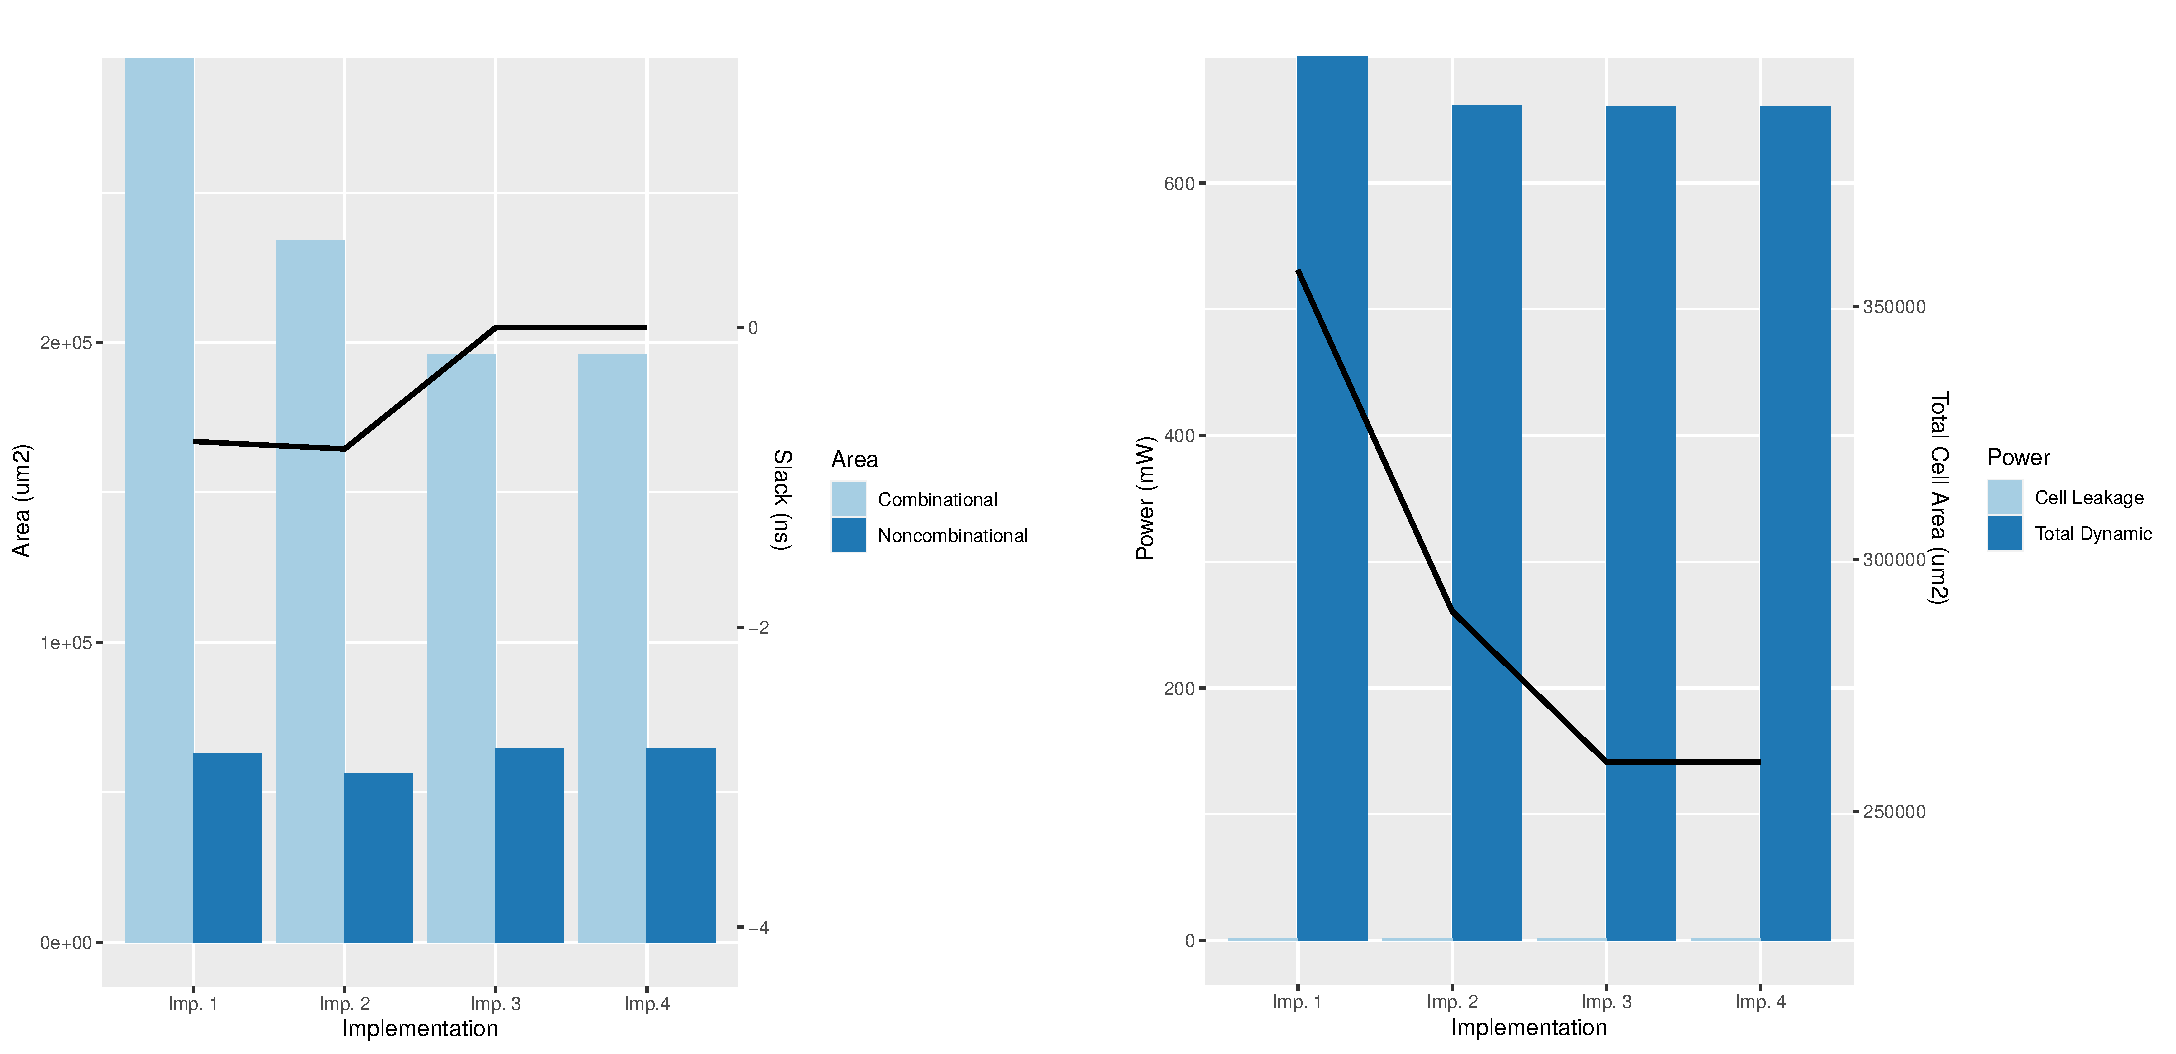
\includegraphics[width=0.85\linewidth]{Diagramas/areaTiempoPower.pdf}
	\caption{Timing-Area-Power evolution.}
	\label{fig:atp}
\end{figure*}


%%%%%%%%%%
%% Seccion
%%%%%%%%%%
%\FloatBarrier
 
\section{Conclusions} \label{sec:conclusions}
This work has presented a VLSI Implementation of a Pipelined 128 points 4-Parallel radix-$2^3$ FFT Architecture via Folding Transformation. The Fourier Transform without folding technique processes 128 entry points of samples which are ordered but its output are disordered and it is necessary a reordering circuit. In the other hand a Fourier Transform with folding technique also needs a reordering circuit in the input. This circuit present an additional area and power consumption to be considered in the final design. 

The folding transformation applied reduce significatively (equal to the folded factor, i.e. 64 times) the number of functional units, and therefore the silicon area, at the expense of increasing the computation time by the same factor. Therefore is necessary to add pipeline cutsets and a careful quantization in order to achieve the required sample period with an acceptable SNR.

Folding technique, in this case, results in an architecture that uses a large number of register, to avoid this is necessary to apply a register minimization technique and allocate data to these registers. The number of registers applying this method is reduced significatively, from  to . This results in a final design with less area and power consumption. %% Calcuar reduccion de registros

The number of DFT points is related with the radix-base, we can write as \textit{radix}-$8$, this representation can be expressed as \textit{radix}-$2^3$ that means we can decompose in smaller radixes with main base-2, an advantage of using a hight radix is reduced the number of multipliers at expense of increase the routing.

Our design has implemented a quantizer block which works with saturation and truncated, the round method was not used because we reached a high SQNR. Lastly a series of optimization were necessary to accomplish the required frequency. The DFT implementation without any optimization level got to work at 166MHz, applying pipelines cutsets and quantization blocks, the final architecture is implementable at the required clock frequency (500 MHz) at the cost of incrementing the numbers of sequential cells. Finally, with the CSD multipliers, is possible to reduce the combinational cells significatively. 



%%%%%%%%%%%%%%
% Bibliografia
%%%%%%%%%%%%%%
\bibliographystyle{IEEEtran}
\bibliography{referenciasFFT}
%%%%%%%%
% FIN
%%%%%%%%
\end{document}
